\documentclass{MMCStyle}
\usepackage{float}
\usepackage{tikz}
\usetikzlibrary{positioning,arrows.meta}
\bianhao{MCB2600843}
\tihao{B}
\timu{基于多源观测的吉隆口岸冰崩—泥石流链关联与条件预测}
\keyword{统一候选关联；床体自重；前向预报；右删失；D8路由}
\newcommand{\paperfig}[4]{\begin{figure}[htbp]\centering\includegraphics[width=#2\textwidth]{#1}\caption{#3}\label{#4}\end{figure}}
\newcommand{\mymunit}[1]{\,\mathrm{#1}}
% 所有表格单元格水平居中；tabularx 的 X 列同时垂直居中。
\renewcommand{\tabularxcolumn}[1]{>{\centering\arraybackslash}m{#1}}
\renewcommand{\arraystretch}{1.10}
\setlength{\extrarowheight}{0.5pt}
\setlength{\emergencystretch}{2em}
\setlength{\intextsep}{5pt plus 1pt minus 1pt}
\setlength{\textfloatsep}{7pt plus 2pt minus 2pt}
\setlength{\floatsep}{7pt plus 2pt minus 2pt}
\setlength{\abovedisplayskip}{4pt plus 1pt minus 1pt}
\setlength{\belowdisplayskip}{4pt plus 1pt minus 1pt}
\setlength{\abovedisplayshortskip}{2pt plus 1pt}
\setlength{\belowdisplayshortskip}{2pt plus 1pt}

\begin{document}
\begin{abstract}
\linespread{1.10}\selectfont
2026年8月26日10:30，吉隆口岸遭受高位冰崩引发的碎屑流—泥石流—山洪链式冲击。本文利用题给多源观测、灾前地形与公开气象产品，建立“关联排序—起动判别—固定发布时刻条件预报—情景传播”的分析框架，并区分可核验的条件结果与尚不可识别的真实触发。

针对问题一，本文从MET、RADM、SOIL、FLUX四类逐时观测固定31项唯一候选，在93个同季参照窗上计算事件前168小时稳健异常，并以Spearman相关簇去冗余。正式前五依次为前期降水指数、净辐射、24小时升温、0.1米土壤含水率和潜热通量，$A$分别为3.829043、2.343641、2.234448、1.487331和1.133226，方向均为事件窗偏高。该结果是单事件环境关联，2025年同类窗口最大$A=3.336817$，不足以证明普适前兆或因果效应。

针对问题二，本文在床面受力中加入床体沿坡自重，区分78条水流控制与6条重力失稳沟道。产流采用完整降雨事件的累计SCS-CN扣损，逐时径流取累计曲线差；事件边界由连续六个零雨小时确认，场初曲线数由前一小时API确定。正式中心线单宽与断面临界流量分别为$q_c=67.588$ m$^2$/s和$Q_c=2.893667\times10^3$ m$^3$/s；事件窗水源峰值202.650 m$^3$/s，最大触发比0.070032，10:00为0.018814，六小时均未越阈。335个厚冰陡坡像元仅是源区候选；冰体强度、裂隙和位移缺失，冰力学状态尚不可识别。

针对问题三，本文固定2026年8月26日08:00当地时发布，只采用06、12、18 UTC三次IFS单次起报及其到达发布端的六小时上界，生成3000个配对成员。短波和降水按原始结束标签对齐到$[t,t+1)$，温湿取两端时点值的梯形均值。源区融水代理的95\%条件区间为09:03:22--10:57:51，即时释放假设下的口岸条件到达区间为09:35:26--11:31:59。真实释放、形成和实际到达尚不能估计，真实预警与覆盖率也未给出；10:30仅落入辅助即时释放区间（1/1），不代表真实覆盖，第三问的真实触发预报仍未完成。08:00融水提示相对锚点有2.5小时信息时差，辅助到达区间相对锚点的提前量为$-1.0332$至$+0.9094$小时；同链沿沟距离为22.924千米。

针对问题四，混合入沟体积为$2.635835\times10^6$ m$^3$。D8基线32.766603分钟到达口岸代理，口岸历史峰深10.085302米，质量相对残差$2.075820\times10^{-15}$、最大Courant数0.188281。16个配置全部终止于26045.494670米分析域末端的右删失，并非自然最大运程；一维基线则在9.336769千米处自然能量停止。数值闭合说明给定离散方案内守恒一致，不构成地形、流变或现场过程验证。

外部气象产品同日降水差异明显，故并列对照而不互相替代。真实泥石流形成真值、现场流深流速及沿程可动库存仍缺失，因此本文给出条件预报及其适用范围，不提供真实灾害95\%覆盖保证。
\end{abstract}
\begingroup
\pagestyle{empty}
\zihao{-5}\linespread{1.00}\selectfont
\tableofcontents
\clearpage
\endgroup
\pagenumbering{arabic}
\linespread{1.20}\selectfont
\pagestyle{fancy}
\section{问题重述与研究设计}
\subsection{任务与需要分开的时间对象}
2026年8月26日10:30，高位冰崩引发的碎屑流、泥石流与山洪链式过程冲击吉隆口岸。此类高位冰崩—碎屑流—泥石流链在喜马拉雅山区多次成灾，其运动性受冰水含量、体积与沿程地形共同影响\cite{schneider2011,iverson1997,richardson2000}。题给时间是口岸冲击锚点，并非源区冰体最初失稳的直接观测。研究需回答四个相连的问题：气象与近地层环境如何关联灾害，何种水源和床面条件达到触发门槛，何时可能触发及如何给出区间与预警，过程在既定地形和参数下如何演化。

令$t_m$为源区融水起始代理，$t_{\mathrm{trig}}$为真实泥石流形成时刻，$t_a^{(0)}$为同一成员在即时释放假设下传播到口岸代理的条件到达时刻，$t_a$为实际到达，$t_p$为固定发布时刻，$t_{\mathrm{hit}}$为题给口岸冲击锚点。冰体失稳可能发生在融水阈值之前，$t_m$与$t_{\mathrm{trig}}$并不等同。为避免同一次事件参与自身验证，本文固定$t_p=$2026-08-26 08:00当地时，先产生源区与口岸配对成员，再以10:30作事后单点核对。四个问题分别回答环境异常、力平衡状态、条件时间区间和传播情景，辅助包含只作单点核对。

地形、物源和水源分别对应能量、物质与触发条件。本文以水源供给与床面起动比值作为主状态，避免把资料条件不同的过程压缩为单一概率；空间模型用于环境对照，运动模型给出条件传播，各问共用同一条公共中心线。

\subsection{资料、来源与用途}
题给八类资料、其发布机构与本文用途见表\ref{tab:data}。来源以机构名与产品名注明，请求参数与产品版本随成果保存。

\begin{table}[htbp]\centering\footnotesize
\caption{题给资料及用途}\label{tab:data}
\begin{tabularx}{\textwidth}{Y >{\hsize=1.10\hsize}Y >{\hsize=1.05\hsize}Y >{\hsize=0.85\hsize}Y}\toprule
附件&资料范围&来源产品&用途与限制\\\midrule
1&2021--2026逐时MET/RADM/SOIL/FLUX&吉隆灾害专题（国家青藏高原科学数据中心）&温湿风廓线、辐射、土壤及湍流诊断；单站代表性有限\\
2&2005--2025周边县日均温（至2025-08）&ERA5-Land逐日统计产品，同上&长期气候背景和同口径积温对照，不代替源区温度观测\\
3&2000--2020四期高程变化&全球冰川高程变化产品，同上&有效像元加权区域背景，均值误差不视为区域均值标准误\\
4&灾前冰川DEM、冰厚、速度&冰川地形与冰厚遥感产品，同上&原生源区积分、源几何与速度重叠旁证\\
5&2020--2023土地覆盖&土地覆被遥感产品，同上&原类码作为分类变量；未确认类码不解释为建设用地\\
6&84处历史灾点面及属性&历史灾点调查数据，同上&沟道临界域、规模排序、历史等效摩擦和面内像元对照\\
7&事件日期研究域DEM&事件区数字高程模型，同上&公共水文地形与路由载体；日期不证明灾前或灾后采集\\
8&第七次县级人口普查&县级普查汇总，同上&县级承灾背景，不空间化为精确暴露人口\\\bottomrule
\end{tabularx}\end{table}

融水面积权重取附件3的RGI6编目多边形与集水区的面积交比，属于编目年代边界，不是2026年实时冰川或积雪范围；高程带代理并列报告但不进入融水。补充的ERA5与MERRA2用于同一UTC+8自然日的产品对照；IFS采用按单次起报保存的06、12、18 UTC档案，分别记录起报时刻、可用上界、有效小时和产品版本。起报可用性表示信息时次满足发布要求，源区冰面实况仍需独立观测确认。

站表共49545行，物理有效46755小时；五层温湿共同有效45577小时，可计算整体理查森数的共同样本44018小时。历史84处灾点中降雨型41、冰水混合型25、冰雪融水型16、冰湖溃决型2，大及特大规模合计9处。该目录每个对象都已发生过灾害，因此无法据此构造完整的发生/未发生样本；DEM相交灾点只是其中一部分，像元样本量不等于独立灾害数量。人口“合计”字段为17536人，只给县级背景，不按均匀密度分摊到狭窄演算走廊。

\subsection{坐标与位置的来源说明}
题面只给“吉隆口岸”，未给实际受灾断面坐标。本文以(85.3826$^\circ$E,28.2826$^\circ$N)为工作点，以(85.3777$^\circ$E,28.2797$^\circ$N)为参考候选，两者平面相距约571米，均按DEM近似位置处理。固定源区、网格、体积和动力参数，仅改变目标点重演：两候选的路线吸附偏移为5.186582和27.40米，D8到达为32.766603和33.90分钟，峰流深10.085302和7.42米，峰速6.601474和8.82米每秒。5.19米是路线吸附偏移，不代表口岸定位精度；两候选间距另行报告。

站点坐标(85.30$^\circ$E, 28.40$^\circ$N)是吉隆沟高寒山区的假定代表点：原始MET、RADM、SOIL与FLUX档案均不含站点元数据。海拔取气压反演值3978.85\,m（标准大气推断），不是实测安装高度；辐射与触发计算取整使用3980\,m，与反演值相差1.15\,m，远小于反演不确定度。太阳能时角计算使用该经度，经度假定误差会线性传播至辐射诊断。

源区、公共注入断面与口岸代理的空间关系见图\ref{fig:study-area}。图(a)只画与DEM相交的历史灾点，域外点不夹取进样本；图(b)中橙星为源区质心，青方块为公共注入断面，红星为口岸工作点，灰叉为参考候选，细线为D8首达路由。源区与口岸均为DEM近似工作点，不是实测断面。

\begin{figure}[htbp]\centering
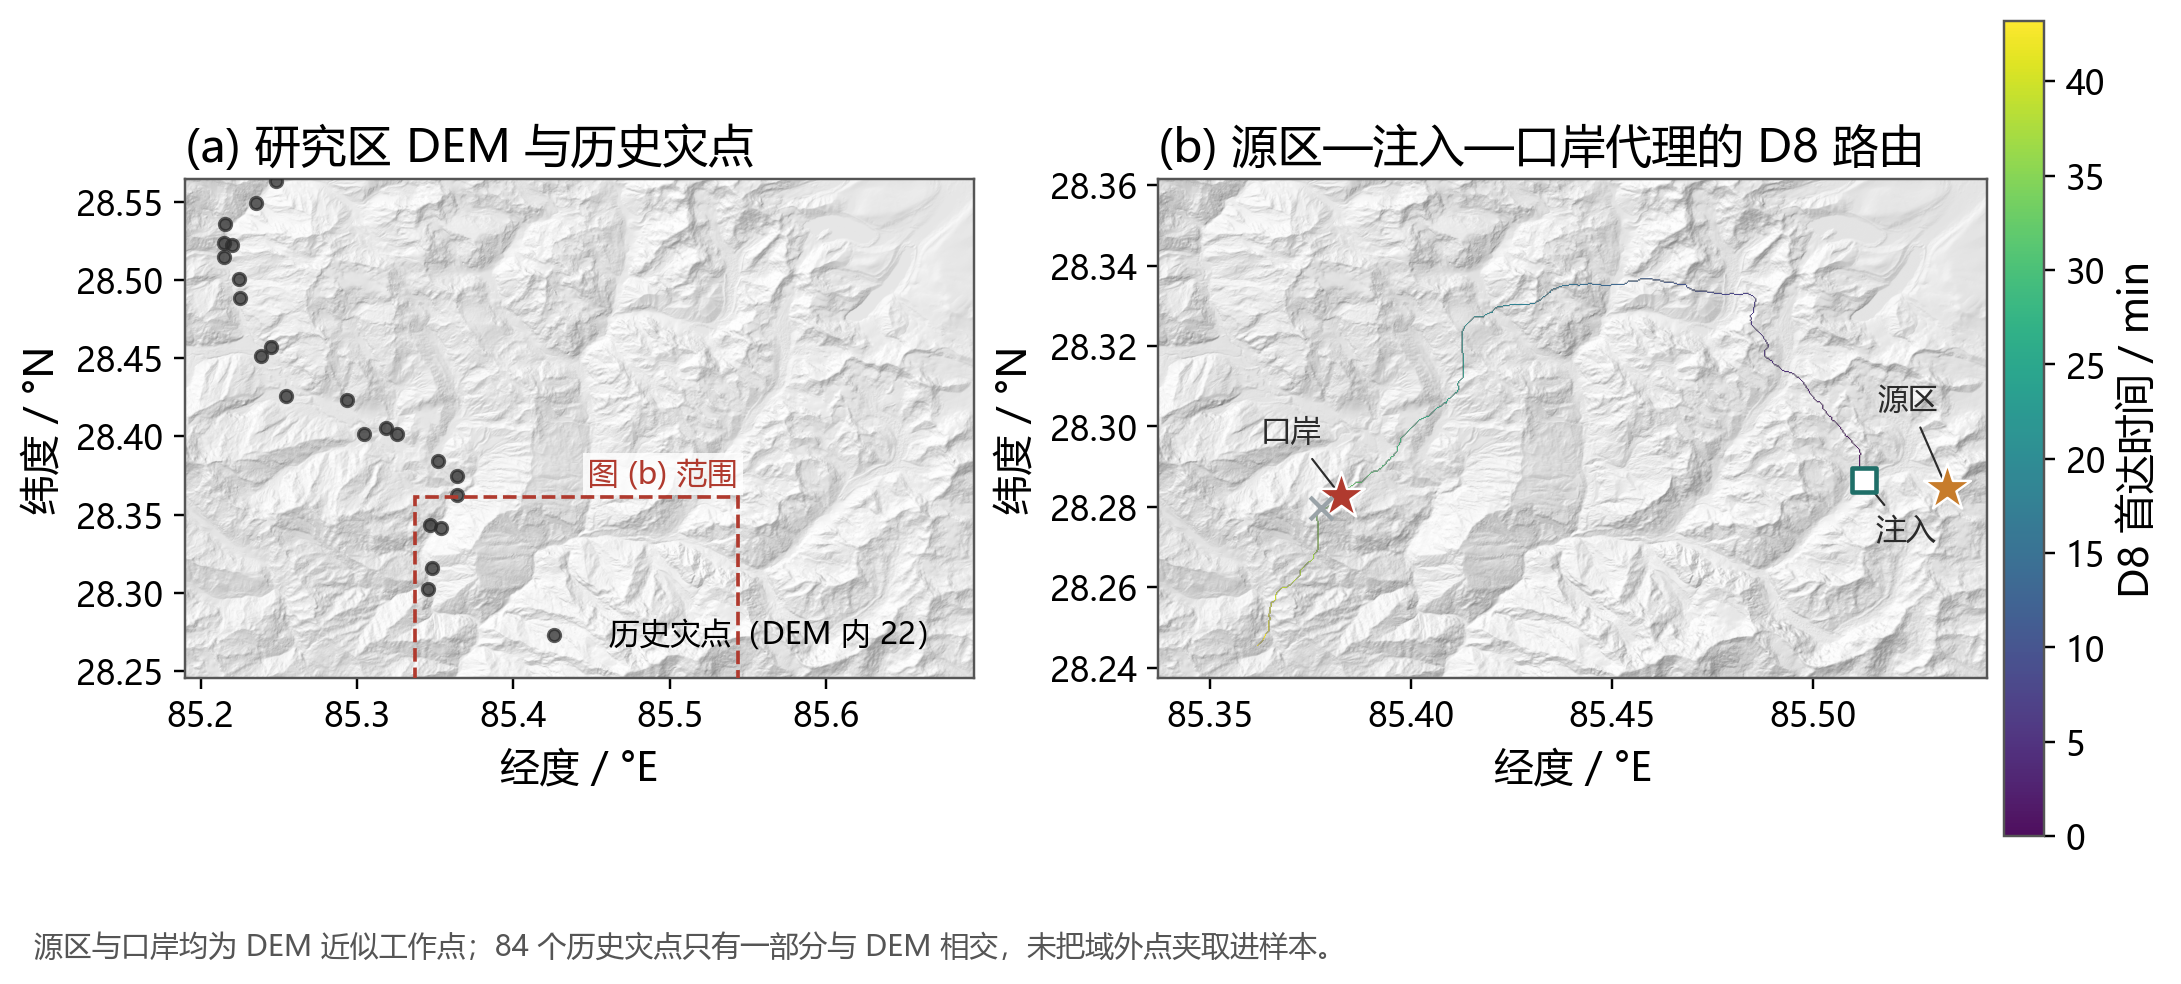
\includegraphics[width=0.96\textwidth]{figures/01_研究区与链式几何.png}
\caption{研究区与链式几何。(a) DEM山影与DEM域内历史灾点；(b) 源区、公共注入断面、口岸工作点与参考候选的D8首达路由。}
\label{fig:study-area}
\end{figure}

\subsection{质量控制和空间一致化}
四类站点资料先按时间戳拼接、去重并重建连续小时轴；哨兵值及不合理物理值置空，质量码释义未充分提供时保守屏蔽非零码。滚动三小时要求三小时均有效，三日小时正积温要求72小时完整；普通自然日聚合至少20个有效小时。日光反照率和晴空指数只在符合日光条件的时段考察，采用有效比例要求而非要求不存在的20小时日照。无观测小时不补零降水或融化；跨缺测的API先重启并保留暖启动期，雨事件分割只把完整观测的干期当间隔，不完整过程的水源状态记为未知。该处理减少可用样本，但避免把缺测误作无雨无融；插补、分位与标准化只在训练集拟合，事件日全日资料仅作描述，不作为事前特征。

空间资料统一以像元中心定位。经纬网格的米制尺寸近似为
\begin{equation}
 d_y=110574|\Delta\phi|,\qquad
 d_x=111320\cos\phi_0|\Delta\lambda|,\quad \phi_0=28.4^\circ.
\end{equation}
主网格南北约30.71米、东西约27.20米，面积约835.27平方米，与900平方米的名义值有明显差异。冰川原生30米UTM网格上的体积先积分再投影，防止多个原生像元落到同一演算格后重复积分；粗化网格原点位于整个块的中心而非左上第一个细格中心。D8选向按真实链接长度比较最大坡降，与后续流量、时间和CFL所用几何一致。

\subsection{外部气象对照}
请求明确指定ERA5、UTC与关闭海拔自动降尺度；NASA POWER请求明确指定UTC。两套逐时响应先转为UTC+8，再按完整24小时汇总事件自然日。
\begin{table}[htbp]\centering\small
\caption{同日界外部气象对照}\label{tab:extmet}
\begin{tabular}{@{}l c c c@{}}\toprule
产品&响应代表高程/m&日均/最高/最低温度/$^\circ$C&日降水/mm\\\midrule
ERA5（Open-Meteo接口）&4322&9.41/13.10/6.40&7.50\\
MERRA2（NASA POWER接口）&4836.18&6.09/11.06/2.43&1.22\\\bottomrule
\end{tabular}\end{table}
两产品事件日降水差异明显，日均温相差约3.32 K。格点代表高程相差约514 m，但温度差与高程差不同向，无法据此反推直减率；粗格点、下垫面与模式偏差未分离，两个接口也不保证统计独立，因此只作并列对照，不替代站点观测。

第三类资料是IFS单次起报。主起报为2026年8月25日18 UTC，并以同日06、12 UTC作模式演化对照；按六小时分发上界，三者最迟分别于25日12 UTC、18 UTC和26日00 UTC可用，均不晚于固定发布时刻。每次取发布前最后完成小时和其后24个有效小时，源区与口岸配对生成1000个成员。普通短波与降水按原始结束标签对齐到$[t,t+1)$，温湿取两端时点值的梯形均值；任一端点缺失则该小时不可评估，不用下一条记录跨过时间缺口。18 UTC口岸格点序列只作独立上下文，不进入主传播链。该流程保证信息时次不晚于发布；模式输出与冰面实况的一致性需另行检验。

站点对照按UTC+8转UTC日，仅保留温降水均有24个有效小时的共同日期；2021--2025分别保留247、363、361、363、214日。2025同窗口站点降水102.00毫米、POWER为742.41毫米；站点年总量不完整，二者不作同口径比较。站点位置、时区与小时标签仍是假设，故只是代表点产品差异。

原始响应、请求参数与产品版本随成果保存；公开站点元数据缺失，真实安装高度及时区仍未知，海拔按反演值处理，不视为实测信息。

\section{问题分析与建模思路}
四个问题共享同一套资料、时间轴和公共几何，但回答对象不同：问题一识别事件前环境异常，问题二判断水源与床面是否达到起动条件，问题三在固定发布时刻给出条件时间产品，问题四在给定体积与地形下演算传播。图\ref{fig:roadmap}给出全文技术路线。

四问共享时间基准、坐标和注入断面，箭头只表示计算依赖；本文将结果分为计算闭合、模型内的条件分布与真实灾害外推三层，结论限于前两层。

\begin{figure}[H]\centering
\begin{tikzpicture}[
  font=\footnotesize,
  base/.style={draw=black!55, rounded corners=2pt, align=center, inner sep=3pt},
  data/.style={base, fill=gray!8, text width=13.8cm, minimum height=1.05cm},
  q/.style={base, fill=teal!7, text width=3.30cm, minimum height=3.55cm, font=\scriptsize},
  outbox/.style={base, fill=orange!8, text width=13.8cm, minimum height=1.2cm},
  arr/.style={-{Latex[length=2mm]}, semithick, draw=black!65}
]
\node[data] (data) at (0,0) {\textbf{题给资料与公共预处理}\\四类逐时观测、DEM、冰川编目、历史灾点、IFS\\时间基准对齐｜质量控制｜公共注入断面｜源区体积};
\node[q] (q1) at (-5.1,-2.65) {\textbf{问题一}\\环境关联\\31项候选\\稳健异常→相关簇\\正式前五};
\node[q] (q2) at (-1.7,-2.65) {\textbf{问题二}\\起动判别\\床面受力→水控/\\重力分支\\事件累计SCS-CN\\→$T(t)$};
\node[q] (q3) at (1.7,-2.65) {\textbf{问题三}\\条件预报\\固定08:00\\3000成员\\$t_m$、$t_a^{(0)}$区间};
\node[q] (q4) at (5.1,-2.65) {\textbf{问题四}\\情景传播\\一维自然停止\\D8路由\\首达、峰值、右删失};
\node[outbox] (ev) at (0,-5.75) {\textbf{结果层次与适用范围}\\计算闭合（单位/状态/账本/CFL）→ 条件成员分布 → 真实触发外推\\真实 $t_r$、$t_f$、$t_a$、真实预警与覆盖率尚未给出};
\draw[arr] (data.south) -- (q1.north);
\draw[arr] (data.south) -- (q2.north);
\draw[arr] (data.south) -- (q3.north);
\draw[arr] (data.south) -- (q4.north);
\draw[arr] (q1.south) -- (ev.north -| q1.south);
\draw[arr] (q2.south) -- (ev.north -| q2.south);
\draw[arr] (q3.south) -- (ev.north -| q3.south);
\draw[arr] (q4.south) -- (ev.north -| q4.south);
\end{tikzpicture}
\caption{全文建模思路与结果层次}\label{fig:roadmap}
\end{figure}


若只读一张图：问题一见图\ref{fig:q1-unified}，问题二见图\ref{fig:q2-trigger}，问题三见图\ref{fig:q3-time-products}，问题四见图\ref{fig:q4-one-d}。

\section{基本假设与符号约定}
\subsection{公共假设与适用范围}
跨问题主要符号见表\ref{tab:symbols}；公共假设逐条列于其后，编号H0-1至H0-9。

\begin{table}[htbp]\centering\footnotesize
\caption{主要符号}\label{tab:symbols}
\begin{tabular}{@{}l l l@{}}\toprule
符号&意义&单位\\\midrule
$\theta_v,Ri_b$&虚位温、整体理查森数&K、无量纲\\
$R_n,H,LE,G$&净辐射、感热、潜热、土壤热通量&W/m$^2$\\
$e_m,m_{src},m_{cat}$&小时能量、源区/流域等效融水&MJ/m$^2$、mm\\
$Q_w,Q_c,q_c$&水源流量、起动流量、单宽起动流量&m$^3$/s、m$^2$/s\\
$T,T_w,P$&触发指数、双通道候选指示、单调相对评分&无量纲\\
$S,n,\tau_y,\mu_H$&比降、糙率、屈服门槛、等效摩擦&1、s/m$^{1/3}$、Pa、1\\
$V_{src},V_{rel},V_{df}$&源冰总量、释放冰量、混合入沟体积&m$^3$\\
$h,v,I$&等效泥深、速度、单位宽动量通量&m、m/s、N/m\\
$t_m,t_{\mathrm{trig}},t_a^{(0)},t_a$&融水起始、真实形成、条件到达、实际到达&h\\
$t_p,t_{\mathrm{hit}}$&固定发布、题给冲击锚点&h\\
$V_{inj},V_{dom},V_{out}$&累计注入、域内、累计出域体积&m$^3$\\
$\mu_{dyn},\kappa,v_0;\ \Delta V_{a,j},B_{a,j}$&动力与节点库存&1、m$^{-1}$、m/s、m$^3$\\\bottomrule
\end{tabular}\end{table}

\begin{enumerate}
\item 题给冲击时刻与附件逐时记录按同一UTC+8标度对齐；IFS原始有效时刻按UTC保存，再转换到当地发布窗。时区元数据缺失，时间对齐仍是主要不确定性。
\item 单站代表同一高程带的大尺度强迫，源区气温按0.5--0.7 K/(100 m)直减率做外推敏感性；不假定局地风和冰体温度已知。
\item 能量余量表示潜在融化能量，闭合缺口不全部归因于实际消融。冰厚、源区比例与物源放大均作为明示场景参数。
\item 模型成员概率、条件分位、确定配置包络和真实事件频率分别命名，避免混合成单一的真实灾害置信区间。
\item 前向链的$t_m$是融水起始代理，$t_{\mathrm{trig}}$是真实泥石流形成时刻；$t_a^{(0)}$由同一成员经固定传播配置得到，是即时释放假设下的条件到达，$t_a$是实际到达。真实释放时刻$t_r$、形成时刻$t_{\mathrm{trig}}$和实际到达$t_a$缺少独立观测，本文暂不给出估计。
\item 过程引擎采用固定地形和集中有限历时注入；侵蚀补给、颗粒分选和堰塞湖溃坝未显式求解。D8终止于分析域时记为右删失；已有漫溢背景作为后续外加源风险，不计入当前释放边界。
\item 历史沟长和扇长按水平投影解释；DEM语义不明时并列冰面与冰下高程假设，不用高分位消除语义歧义。
\item 有限库存对照中的沿程节点与库存均为合成机制情景，不代表已确认的物源点；其速度是团块沿固定路线的条件速度，不等于真实前锋速度或流深。
\item 口岸工作坐标为DEM量图近似位置（28.2826$^\circ$N, 85.3826$^\circ$E），与参考候选相差约0.6\,km；源区至注入断面水平距离2041.449\,m，公共注入至口岸代理中心线20882.237\,m。站点坐标为假定代表点，海拔取气压反演值3978.85\,m。上述位置均按DEM近似，不是实测安装或受灾断面数据。
\end{enumerate}

这些假设由现有资料条件决定；若与观测冲突，本文保留原设定并报告偏差，不通过调整起点、剔除成员或放宽阈值追求表面一致。阈值用于比较，进一步率定仍需独立灾害目录和现场观测。

全文小时步上的mm是该小时水当量深，不额外再除一小时；流量转换统一使用$1\mymunit{mm}\times1\mymunit{km^2}/1\mymunit{h}=1/3.6\mymunit{m^3/s}$。同一符号在日累计时附日下标，避免把全期累计能量与单日门槛相比较。

\section{问题一：近地层结构、天气过程与统一关联排序}
\noindent\textbf{本问结论：}在31项固定候选中，API是唯一$A>3$的候选（3.829）；净辐射、24小时升温、0.1\,m土壤含水率和潜热通量随后，$A$为1.133--2.344。该结果是单事件环境关联，不是因果效应或发生概率；2025同类窗最大值3.337只作同类日期对照，不构成非灾样本。

\subsection{问题口径与分析范围}
题面要求依据MET、RADM、SOIL与FLUX四类逐时观测，分析高寒山区近地层结构、天气过程和极端事件，并给出与本次泥石流关联最高的五个特征。本文将诊断与排序分开：前者描述边界层和能量过程的结构，后者在固定候选池和同季匹配背景下判断本次冲击前哪个环境量最异常。目前只有一次确证事件，且没有完整非灾目录，因此结果限于环境关联排序，不涉及灾害发生概率、总体因果效应或分类AUC。正式前五指：在统一候选池中，按事件前环境窗相对同季历史窗的稳健异常、经相关簇去冗余后的五个代表量。

\subsection{五层静力订正与稳定度诊断}
梯度观测高度为1、2、4、10、20米。MET表头只给一个Pressure字段，未给气压传感器参考高度；FLUX的PA又缺少安装与校准信息。若把整层气压视为常数，层间压降会进入位温、虚位温和整体理查森数，使稳定度混入压力假设。本文以2米为参考高度的显式工作假设，保持五层温湿与MET气压共同有效，按
\begin{equation}
\frac{\mathrm d\log p}{\mathrm dz}=-\frac{g}{R_dT_v},\qquad
T_v=(T_C+273.15)(1+0.61q)
\end{equation}
作逆虚温分段梯形积分，更新层压三次。每次用当前层压重算比湿、位温和虚位温，再以第三次层压统一重算全部诊断量；第二、三次更新差的中位约$9.1\times10^{-12}$ hPa，最大约$6.5\times10^{-11}$ hPa，说明迭代已收敛，但不构成传感器误差界。

五层共同有效45577小时，占全部49545小时的91.99\%；仅3个可用小时因五层要求被新增剔除。可计算整体$Ri_b$的共同样本为44018小时。位温、虚位温与整体理查森数取
\begin{equation}
\theta_z=T_{K,z}\left(\frac{1000}{p_z}\right)^{0.2857},\quad
\theta_{v,z}=\theta_z(1+0.61q_z),\quad
Ri_b=\frac{g}{\bar\theta_v}
\frac{(\theta_{v,20}-\theta_{v,2})(20-2)}
{(u_{20}-u_2)^2+(v_{20}-v_2)^2},
\end{equation}
其中饱和水汽压采用Bolton式，温度入口为摄氏、位温入口为开尔文，两个入口不混换。切变平方小于$10^{-6}\ \mathrm{m^2/s^2}$时屏蔽并报告比例，不强行赋有限值。

静力订正会实质改变稳定度分类。与“全层同一气压”的对照相比，44018个共同小时中有9016个分类改变，占20.48\%；同压对照的$Ri_b$中位为$-0.0636$，订正后为$-0.0294$，$p05$--$p95$为$-4.343$--$19.647$。订正后的五级频率依次为强不稳定0.2441、不稳定0.3856、中性0.0531、稳定0.0852、强稳定0.2320。两组使用同一批小时，只改变层压处理，故差异不是由样本变化制造的。

逆温按实际温度梯度而非位温梯度定义，操作阈值为0.05 K/(100 m)。总逆温频率为0.4111，夜间0.6007、白天0.2079，呈现夜间辐射降温、白天地表受热增强混合的相对日变化。有效厚度以2米为底层，依次检查2--4、2--10、2--20米的首个$Ri_b=0.25$交点；已出现交点的中位为4米，交点层顶以4米最多（7698小时），10米2392小时、20米1437小时；31116小时在20米内仍未达到0.25，按右删失记录；20米是观测上限，不是真实边界层高度。

\begin{figure}[htbp]\centering
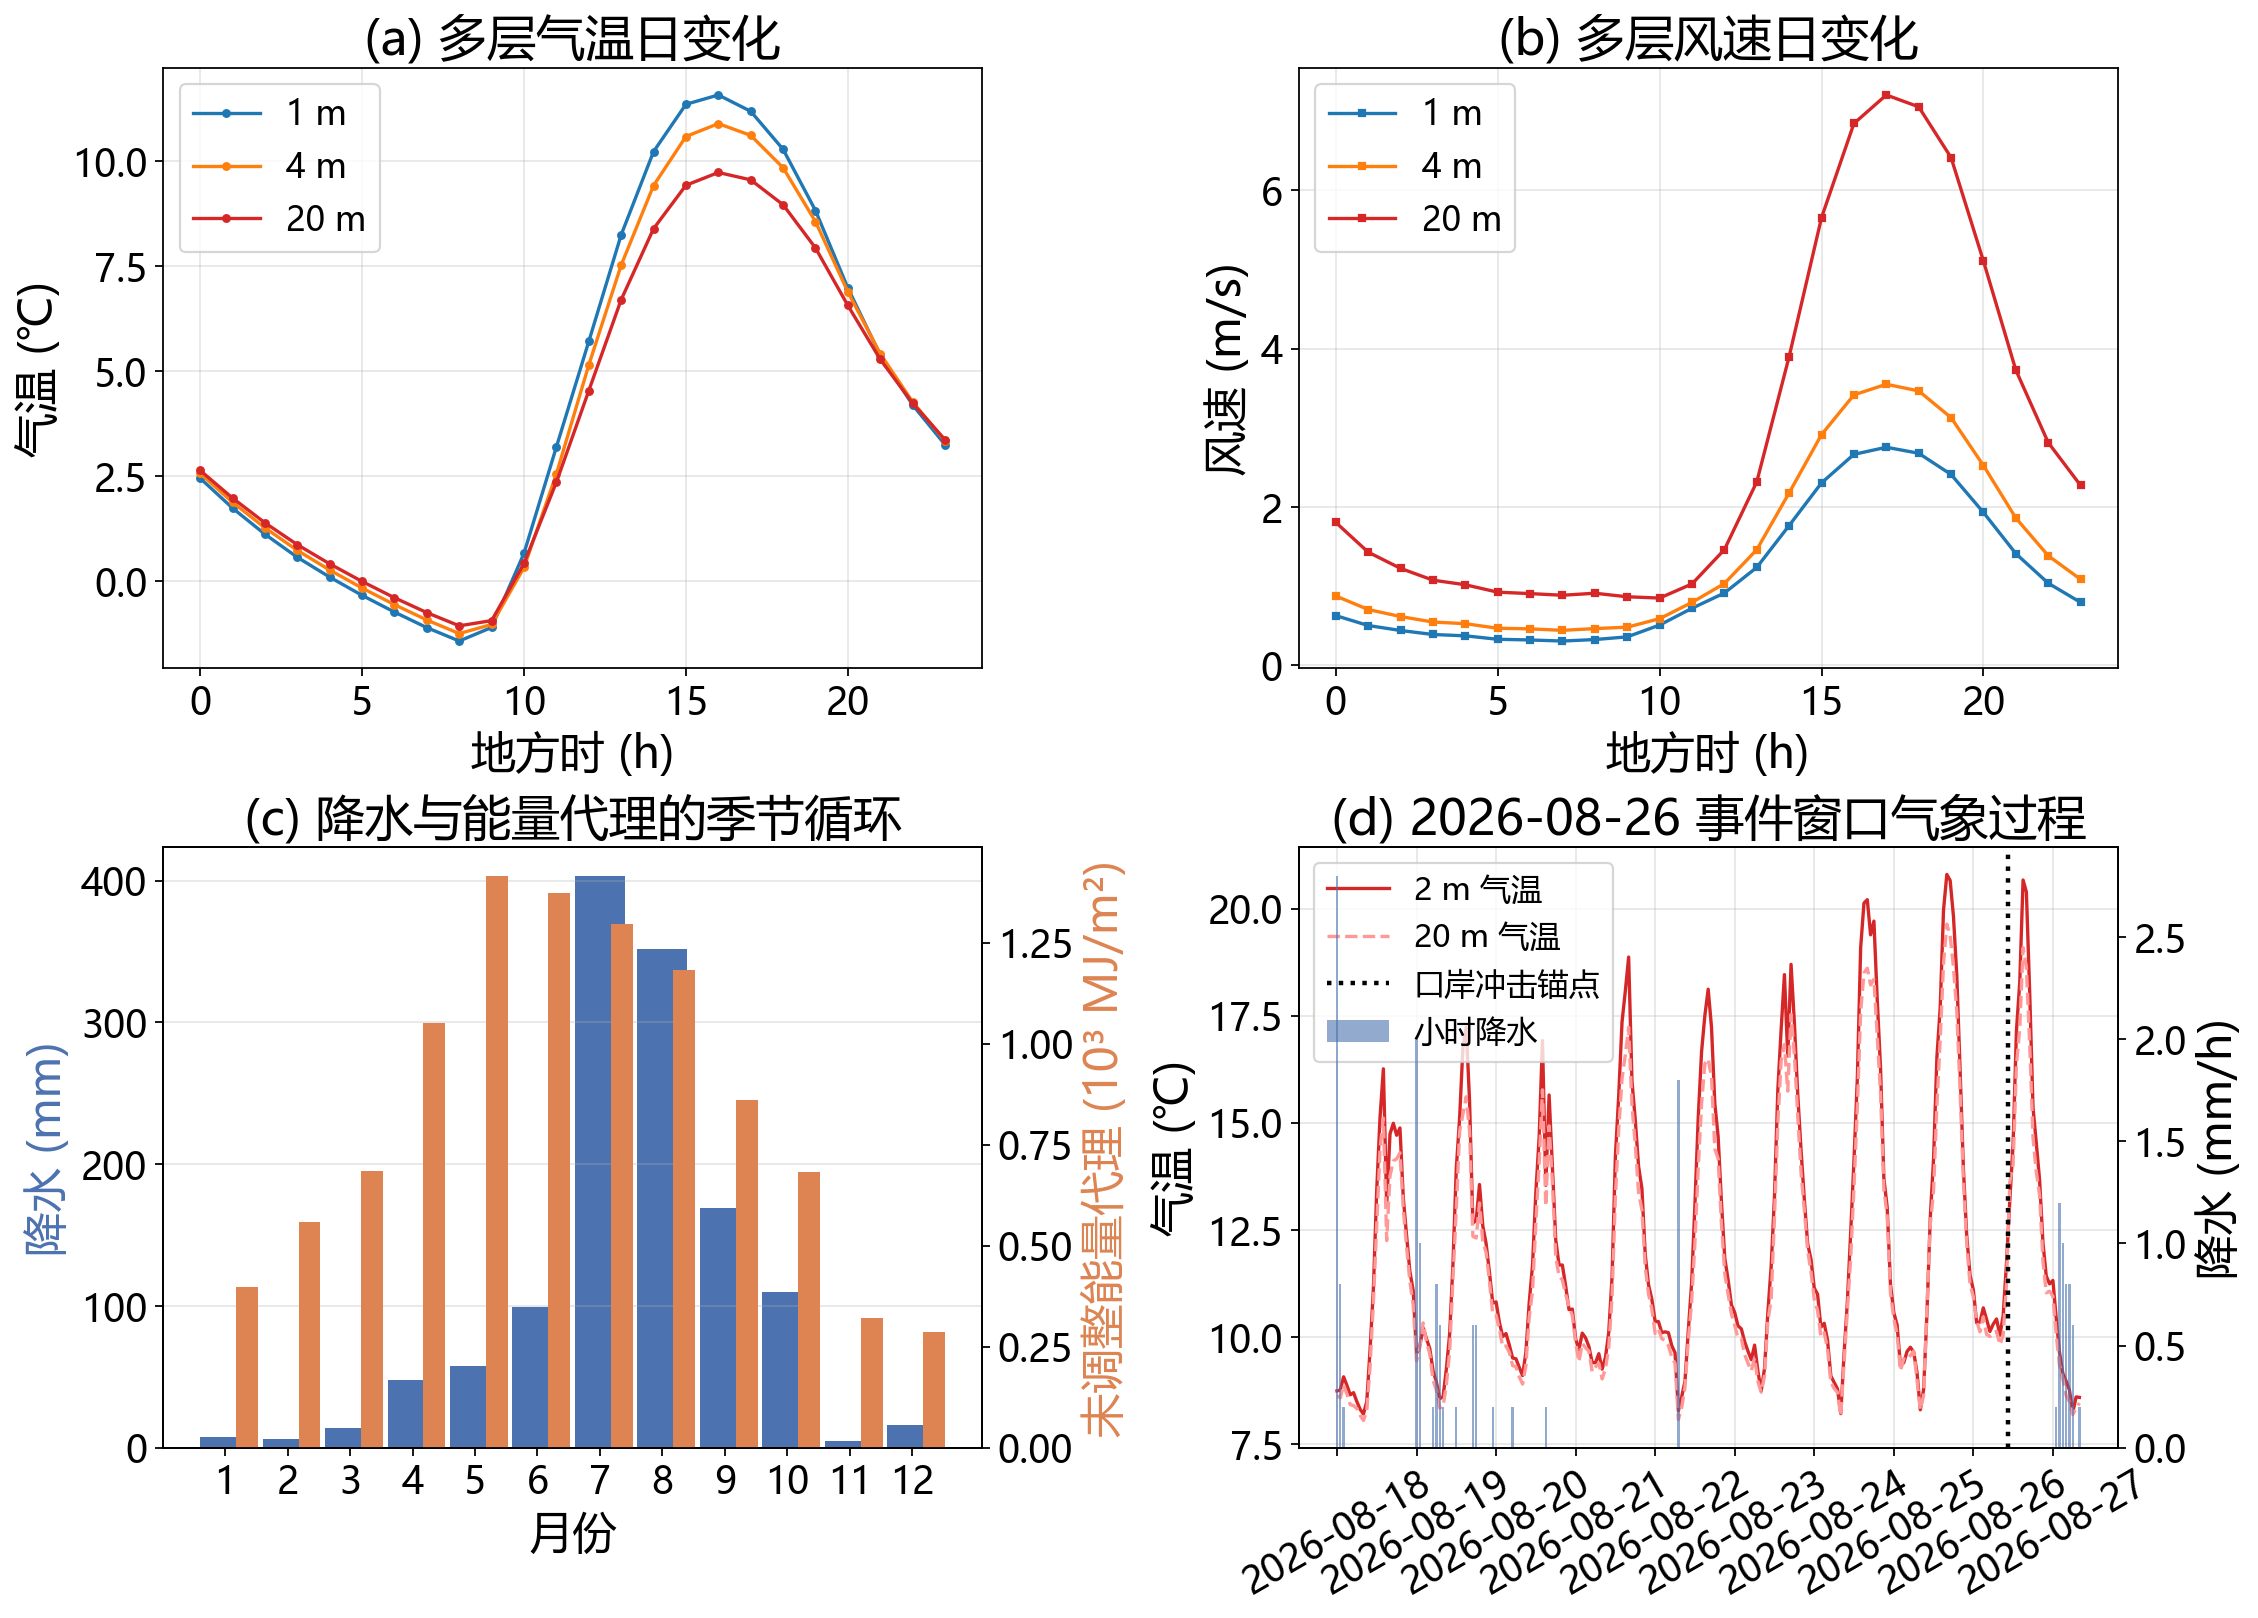
\includegraphics[width=0.78\textwidth]{figures/01_边界层结构.png}
\caption{近地层日变化与事件窗口}
\label{fig:boundary}
\end{figure}

图中季节能量为代理量，事件全日曲线仅用于描述。这些频率受质量码、夜间弱湍流缺测和20米观测上限限制。图\ref{fig:boundary}的日变化是多年统计，不是单个事件的独立控制实验；夜间逆温常见，也不等于每次泥石流都由逆温触发。图\ref{fig:hydrostatic}比较同一批小时上“整层同一气压”与1、2、10、20米参考高度订正的结果，分类改变集中在中性与稳定边界附近。参考高度是工作假设，差异不反映真实传感器高度。

\paperfig{figures/01_静力订正敏感性.png}{0.78}{静力订正敏感性}{fig:hydrostatic}

\subsection{辐射收支、天气过程与极端事件}
用四分量辐射构造$R_n=R_{sd}-R_{su}+R_{ld}-R_{lu}$，反照率只在短波足够大时使用。未调整的小时潜在融化能量为
\begin{equation}
e_m=0.0036[R_n-G-(H+LE)]^+\quad[\mathrm{MJ/m^2\,h^{-1}}],
\qquad [x]^+=\max(x,0).
\label{eq:energy}
\end{equation}
正部约定排除夜间净冷却被误当作负融水。取2021--2025年、$R_n-G>20\ \mathrm{W/m^2}$且四项共同有效的12125小时，回归斜率$\beta_{EC}=0.3343$，而闭合比
\begin{equation}
C=\frac{\sum(H+LE)}{\sum(R_n-G)}=0.4515
\end{equation}
该比值描述能量账本比例，其不确定度由块重采样估计，回归斜率标准误不适用于此。以完整训练年为块重采样500次，$C$的95\%区间为$[0.4441,0.4619]$，无效重采样比例为0。事件相关三日未调整能量合计32.19 MJ/m$^2$；点闭合比调整后为9.35 MJ/m$^2$，两端比值情景约8.85--10.06 MJ/m$^2$。变化远大于数值舍入误差，故基准保留未调整值，调整值只作结构敏感性，不把两者平均为“更真实的消融量”。

将五层气温、湿度、风速和气压组成16维向量，在2021--2025年标准化后作SVD。前三主成分解释方差为53.997\%、30.716\%、11.173\%，达到85\%需要3个模态。第一主成分与融化能量相关0.4304，与24小时降水相关$-0.0964$，故不宜简单命名为降雨模态。另以训练期90\%分位划分强降水、强消融、二者同超和平缓四类；34782个有效小时的比例依次为9.16\%、8.82\%、1.43\%、80.58\%，缺测小时保持未知，不归入平缓型。

极端量采用12小时游程去丛集后的广义帕累托分布。令$Y=X-u>0$，则
\begin{equation}
F_Y(y)=1-\left(1+\xi y/\sigma\right)^{-1/\xi},\qquad
x_T=u+\frac{\sigma}{\xi}\left[(T\lambda_y)^{\xi}-1\right],
\end{equation}
其中$\lambda_y$为独立过程的年次数，暴露年数按有效小时折算；$\xi=0$取连续极限，$\xi<0$时返回水平还须低于有限上界$u-\sigma/\xi$。小时降水97\%分位落在0，正雨小时全部进入尾部；短记录下2年、5年水平只是拟合描述。复合极端主要集中在6--9月，但因缺少多事件起动目录，本文不估计因果风险倍数。

\subsection{31项统一候选关联模型}
正式候选池在求值前固定为31个唯一变量键，家族构成为MET 19项、RADM 5项、SOIL 3项、FLUX 4项。候选覆盖原始气象、温湿与风廓线派生量、辐射能量、土壤状态和湍流通量。小时降水$P$与3小时、24小时累积量是不同时间尺度，不按别名删除；$P_{\max,1h}$与$P$的数值及缺测掩膜逐行相同，只保留$P$。晴空指数和反照率仅白昼有效，固定后分别只有84与82个目标小时，低于135小时门槛；冻融量则因参照窗不足或稳健尺度为零，三项均保留在候选字典中并标为不可排名，其余28项进入正式评分。

题一关联截止为2026-08-26 00:00（非题三08:00业务发布），最后可用标签为前一日22:00。主窗为
\begin{equation}
\mathcal W_{168}=[2026\text{-}08\text{-}18\,23{:}00,
2026\text{-}08\text{-}25\,22{:}00],
\end{equation}
按小时标签$[t,t+1)$计共168小时；72小时敏感性窗取最后72个标签。目标窗和每个候选的参照窗均要求至少达到80\%有效，即主窗不少于135小时，缺测保持为空，不插值或补零。主参照为2021、2023、2024年同积日前后15日内的93个发布窗；2022年因FLUX摩擦速度和观测湍流动能缺测，没有窗口通过共同覆盖门槛，故该年进入逐时相关计算但不进入窗口参照。2025年同历日窗作为无灾害真值的同类日期对照。

对候选$j$和窗长$L$，令目标窗均值为$m_{j,L}$，参照窗均值的中位数和稳健尺度分别为
\begin{equation}
b_{j,L}=\operatorname{median}_r m^{(r)}_{j,L},\qquad
s_{j,L}=1.4826\operatorname{median}_r
\left|m^{(r)}_{j,L}-b_{j,L}\right|,
\end{equation}
并定义$\Delta_{j,L}=m_{j,L}-b_{j,L}$、$Z_{j,L}=\Delta_{j,L}/s_{j,L}$、$A_{j,L}=|Z_{j,L}|$。MAD为零时采用预先规定的$IQR/1.349$回退；回退值仍为零则不排名。同时报告原始单位差、有符号方向和经验尾秩
\begin{equation}
p^{\mathrm{tail}}_{j,L}=
\frac{1+\sum_r\mathbf 1[A^{(r)}_{j,L}\ge A_{j,L}]}{N_{ref}+1},
\end{equation}
该尾秩只是已选参照中的描述量，不是独立检验$p$值；主排序只按$A$降序。

去冗余在2021--2024年6--9月逐对计算Spearman相关。一对候选至少共享200个有效小时才可判定边，$|\rho_s|>0.8$时连边，再取完整连通簇；全部465对均达到共同有效门槛，共同有效小时数的中位为11208小时。31项候选合并为16个连通簇，其中13个含可排名代表。每簇在168小时主评分中只保留$A$最大的可排名候选进入展示，其他成员和完整统计量继续保存。相关簇只解决展示重复，强相关只表示统计关联，不表示机制相同。

\subsection{正式前五与解释}
去冗余后的正式前五见表\ref{tab:q1-top5}，所有方向均为事件窗偏高。前五直接构成题面所问的统一关联排序；代理标签榜和CRITIC榜不再占用“本题答案”。

\begin{table}[htbp]\centering\small
\caption{事件前168小时统一关联榜前五}\label{tab:q1-top5}
\begin{tabular}{@{}c l l c c c@{}}\toprule
次序&变量&家族&$\Delta$（原单位）&$A$&经验尾秩\\\midrule
1&API（前期降水指数）&MET&14.484464&3.829043&0.0106\\
2&$R_n$（净辐射）&RADM&19.928307&2.343641&0.0745\\
3&24小时升温&MET&0.312310&2.234448&0.0957\\
4&VWC（0.1米土壤含水率）&SOIL&0.035295&1.487331&0.1809\\
5&LE（潜热通量）&FLUX&12.883223&1.133226&0.1724\\\bottomrule
\end{tabular}
\end{table}

表中$A$的前三项未舍入值为3.8290425800714973、2.3436406435384014和2.2344476050143953；后两项为1.4873309113872661和1.1332257049823602。

\begin{figure}[htbp]\centering
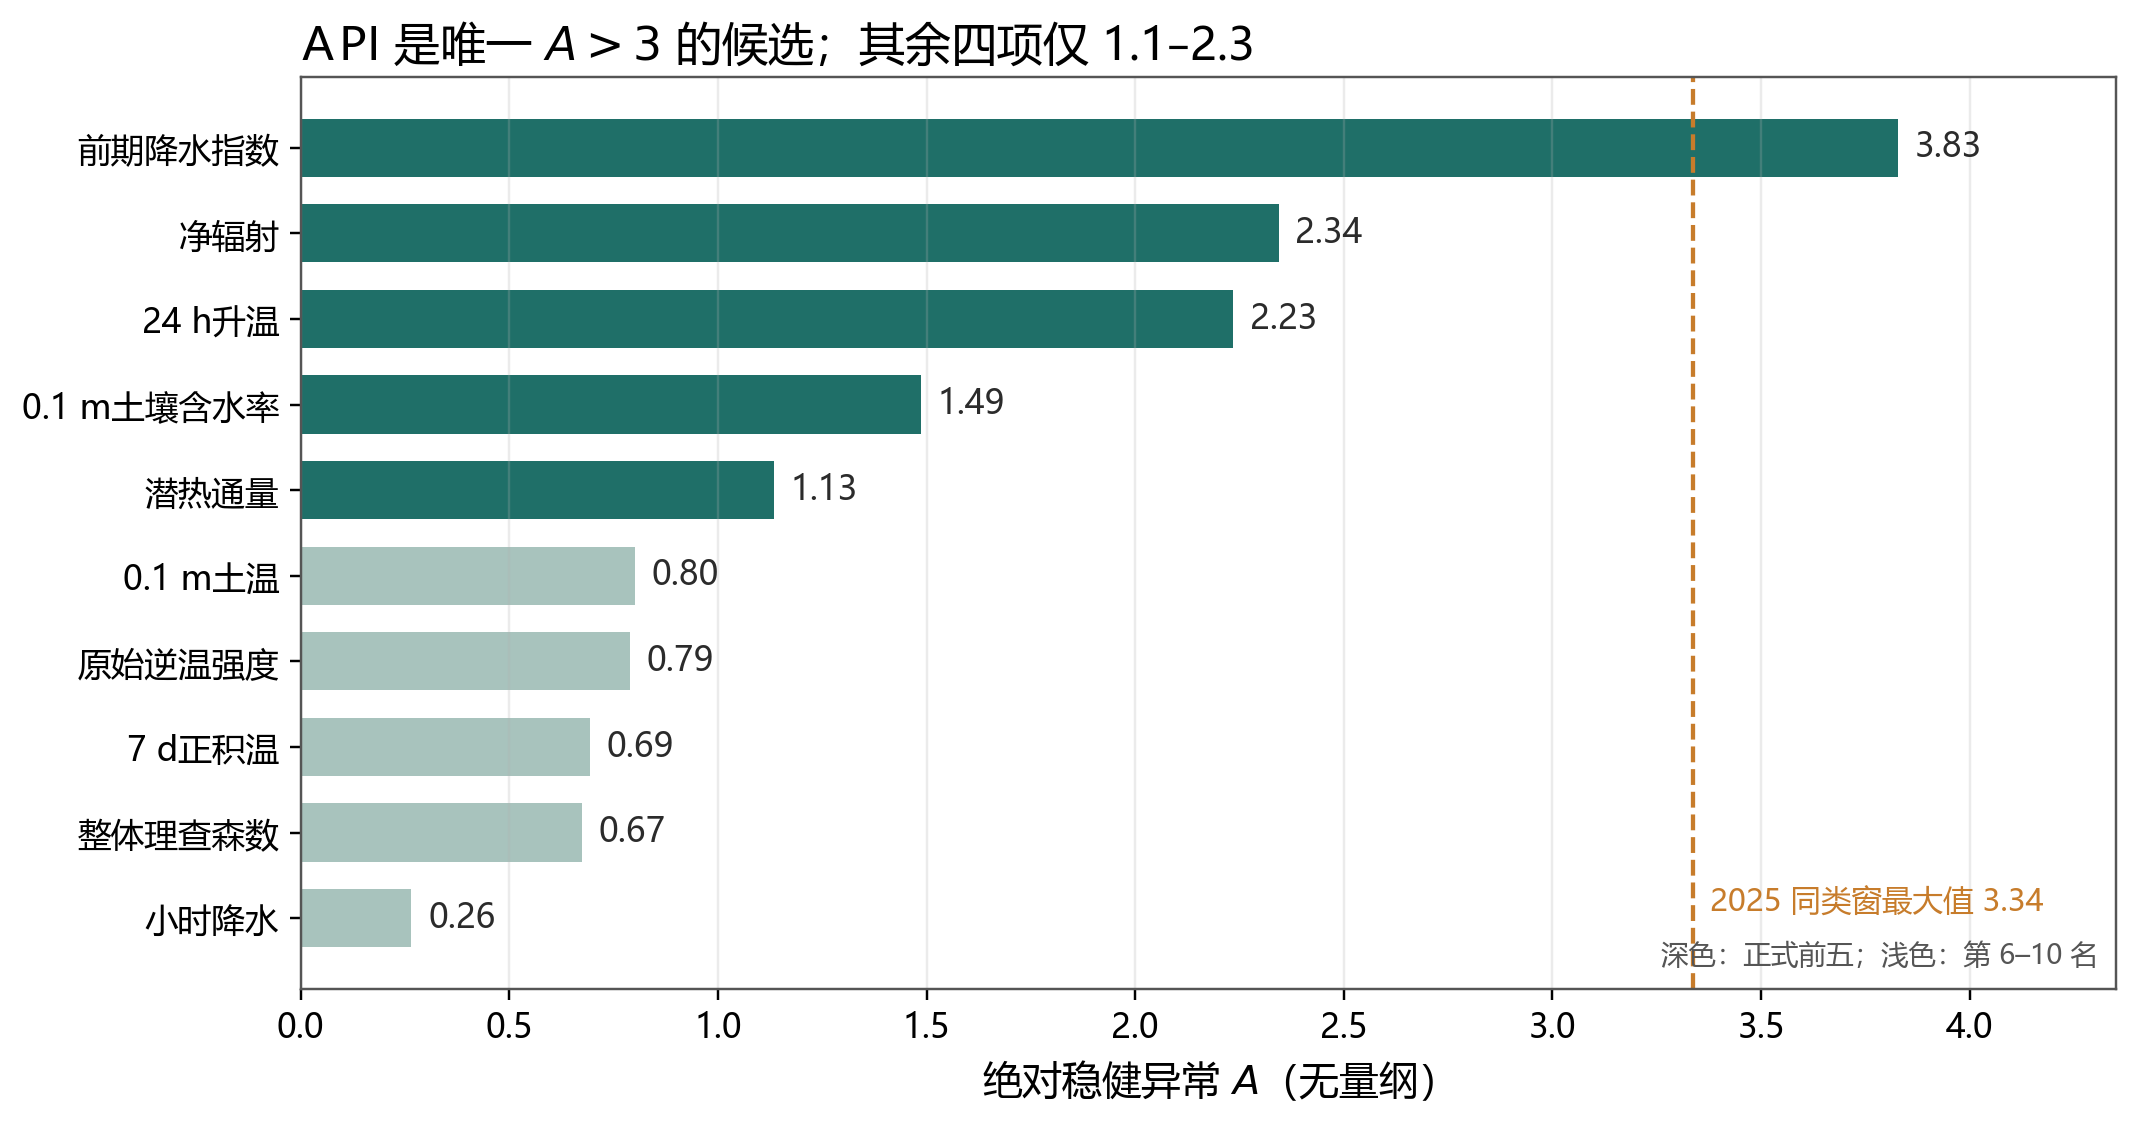
\includegraphics[width=0.90\textwidth]{figures/01c_统一候选关联.png}
\caption{事件前168小时相关簇代表的前10项。深色为正式前五，橙色虚线为2025同类窗最大值。}
\label{fig:q1-unified}
\end{figure}

图\ref{fig:q1-unified}只展示前10项，避免把31项全表压进正文；颜色只区分正式前五与其余候选，虚线给出同类日期参照，不表示机制独立性。完整31项及相关簇成员见附录图\ref{fig:q1-full}。

API的事件窗均值为23.492 mm，参照中位为9.008 mm，绝对差14.484 mm，是唯一$A>3$的候选，说明本次过程前存在较持续的降水记忆。$R_n$的事件窗均值为158.479 W/m$^2$，参照中位为138.551 W/m$^2$；其所在相关簇同时含2米温湿、风切变、短波、消融能量及部分湍流通量，应把它理解为近地层能量状态的代表，而不是独立机制。24小时升温均值为0.294 $^\circ$C，参照中位为$-0.019\ ^\circ$C，反映事件窗内快速增温。0.1米土壤含水率均值0.1271，高于参照中位0.0918，表示浅层土壤水分偏湿；LE均值54.917 W/m$^2$，高于参照中位42.033 W/m$^2$。后四项的$A$均小于1.5，异常幅度明显小于API。

窗长敏感性保留了“降水记忆和升温”这一信号：72小时去冗余前五为小时消融有效能量、API、$Ri_b$、24小时升温和降水，与168小时前五重合API和24小时升温两项。留一年检查亦不完全稳定：省略2021、2023、2024年时前五重合数分别为4、3、3项；省略不同年可能使API与7日前期降水互换代表，但相关簇成员关系仍在。2025年同历日对照的最大$A=3.336817142622748$，低于本次正式头项3.8290425800714973；这表明本次头项不低于该同类日期，但单个2025日期不足以构成确证非灾样本。

\subsection{构造性对照与适用限制}
旧的26项代理榜以水源代理$Q_w$的90\%分位为标签，前五为净辐射、饱和水汽压差、2米气温、API和24小时累积降水，2021--2024训练、2025留出的AUC为0.9902。该高分首先说明水文代理可由其驱动项重建；净辐射、温度、降水和API又直接参与标签或供水构造，其排序不构成独立发现。与代理榜前五相比保留4项，全榜$\tau=0.7169$；CRITIC三列反映事件异常、强水源日判别与触发耦合之间的冲突，三列共享观测，只用于方法比较，不构成独立数据验证。因此两榜定位为构造性对照，不是本文正式前五。

正式榜的适用范围如下。第一，它是单事件环境关联；没有非灾目录，$A$不用于转换发生概率、风险比或普适排序。第二，93个参照窗来自三个有效年份，年际样本有限；尾秩受窗口重叠影响，不作为独立$p$值。第三，API、$R_n$、消融能量和LE与问题二水源模型共享观测或物理构成，榜上位置不表示独立预测能力。第四，站点代表局地近地层，不代表源区冰温和县域空间梯度。第五，相关簇去冗余只影响展示；被合并变量仍有物理意义，完整31项排序和相关边随成果保存。正式结论是：在固定候选池和同季匹配方案下，API最异常，净辐射、24小时升温、浅层土壤含水率和潜热通量随后；这五项用于解释本次事件前的环境组合，不足以单独证明因果或预测未来泥石流。

\section{问题二：床面临界条件与多尺度触发评估}
\noindent\textbf{本问结论：}84条历史沟道中78条水流控制、6条重力失稳；正式中心线$Q_c=2.893667\times10^3$ m$^3$/s，事件窗水源峰值202.650 m$^3$/s、$T_{\max}=0.070032$，六小时未越阈。该负结果说明当前无黏聚、无超孔压的水控链条没有把冰崩链识别为水力越阈事件；冰体强度、裂隙和位移缺失，冰力学状态仍不可识别。

\subsection{问题定义与适用边界}
水源异常与床面能否起动不是同一命题。本文把连续水力型沟道与冰崩链分开：前者用无黏聚、无超孔压的饱和松散床层给出门槛；后者在现有资料下输出条件状态，不用一次事件的时间窗反向标定系数。附件6的84个对象均为已发生灾点，不含确证非灾沟道，因此本文比较已发生对象之间的门槛和规模，不估计发生概率、真实空间AUC或误报率。

床层竖直厚度记为$z_b$，水深垂直床面，应力和门槛统一按单位坡面面积报告。取水密度$\rho_w=1000\ \mathrm{kg/m^3}$、固相密度$\rho_s=2650\ \mathrm{kg/m^3}$和床体固相体积分数$C_v^{(b)}$，有
\begin{equation}
\rho_{\mathrm{sat}}=C_v^{(b)}\rho_s+(1-C_v^{(b)})\rho_w,
\qquad
\Delta\rho=\rho_{\mathrm{sat}}-\rho_w=1650C_v^{(b)}.
\end{equation}
若$C_v^{(b)}\notin(0,1]$、$\Delta\rho\le0$、$z_b\le0$或比降无效，力学分支记not\_evaluable，不用零密度差继续产生正门槛。

\subsection{完整受力、临界链条与三个分支}
令$S=\tan\theta$。水流在床面产生的拖曳应力、床体沿坡自重和有效法向摩擦抗力分别为
\begin{equation}
\tau_w=\rho_wgh\sin\theta,\qquad
\tau_{g,\parallel}=\Delta\rho\,gz_b\sin\theta\cos\theta,\qquad
\tau_r=\Delta\rho\,gz_b\cos^2\theta\tan\varphi.
\end{equation}
最低无黏聚、无超孔压模型的起动条件为
\begin{equation}
\tau_w+\tau_{g,\parallel}\ge\tau_r.
\end{equation}
控制水流状态时，水流所需承担的净抗力为
\begin{equation}
\tau_{wc}=\Delta\rho\,gz_b\cos^2\theta
\left(\tan\varphi-\tan\theta\right).
\label{eq:tauwc}
\end{equation}
取无量纲容差$\varepsilon_S=10^{-6}$，按$S$与$\tan\varphi$的关系划分：
\begin{equation}
\begin{cases}
\text{水流控制},&S<\tan\varphi-\varepsilon_S,\\
\text{摩擦平衡},&|S-\tan\varphi|\le\varepsilon_S,\\
\text{重力失稳},&S>\tan\varphi+\varepsilon_S.
\end{cases}
\end{equation}
因此$S>\tan\varphi$为重力失稳，零水流门槛不等于安全；$S=\tan\varphi$为摩擦平衡，表示净水流抗力为零，同样不属于“稳定”或“已触发”状态。水流控制时，临界水深、单宽临界流量和断面临界流量依次为
\begin{equation}
h_c=\frac{\tau_{wc}}{\rho_wg\sin\theta},\qquad
q_c=\frac{h_c^{5/3}S^{1/2}}{n_m},\qquad
Q_c=q_c\frac{B}{\kappa_B},
\label{eq:qcrit}
\end{equation}
其中$n_m$为Manning糙率，$B$为全沟宽，$\kappa_B$为全沟宽与有效过流宽度之比。零门槛分支令$h_c=q_c=Q_c=0$，并保留其机械状态；只有水流控制且$Q_c>0$时才定义有限触发比$T=Q_w/Q_c$，避免零除和无意义的无穷大。

基准参数取$C_v^{(b)}=1050/1650=0.636364$、$z_b=1.0$ m、$\tan\varphi=0.55$、$n_m=0.06\ \mathrm{s/m^{1/3}}$、$\kappa_B=6$。中心线沟宽按$B=\min\{9\sqrt{A_{km^2}},400\}$ m取为256.881 m。正式中心线比降为0.10185，代入上式得$h_c\approx4.596$ m、$q_c=67.587745\ \mathrm{m^2/s}$、$Q_c\approx2.893667\times10^3\ \mathrm{m^3/s}$。这些是带明示工程参数的模型门槛，不是现场设防标准。由式\ref{eq:qcrit}可见，$q_c$随$z_b$和$\Delta\rho$按约$5/3$次幂放大，随$n_m$近似反比变化；一次事件不能分别识别床厚、摩擦角、宽度和糙率。

对84条历史沟道，正式状态为78条水流控制、6条重力失稳，无摩擦平衡和不可评估对象。78条正门槛沟道的总起动流量中位为63.261 m$^3$/s，四分位区间为12.614--228.441 m$^3$/s。床体固相分数取0.15、0.636364、0.80时，正门槛中位分别约5.690、63.261、92.635 m$^3$/s，说明床体密度假设本身可改变门槛量级。图\ref{fig:q2-critical}给出状态分支与78条正门槛沟道的$Q_c$分布；床厚、摩擦角、宽度和糙率的敏感性见本节数值。

\begin{figure}[htbp]\centering
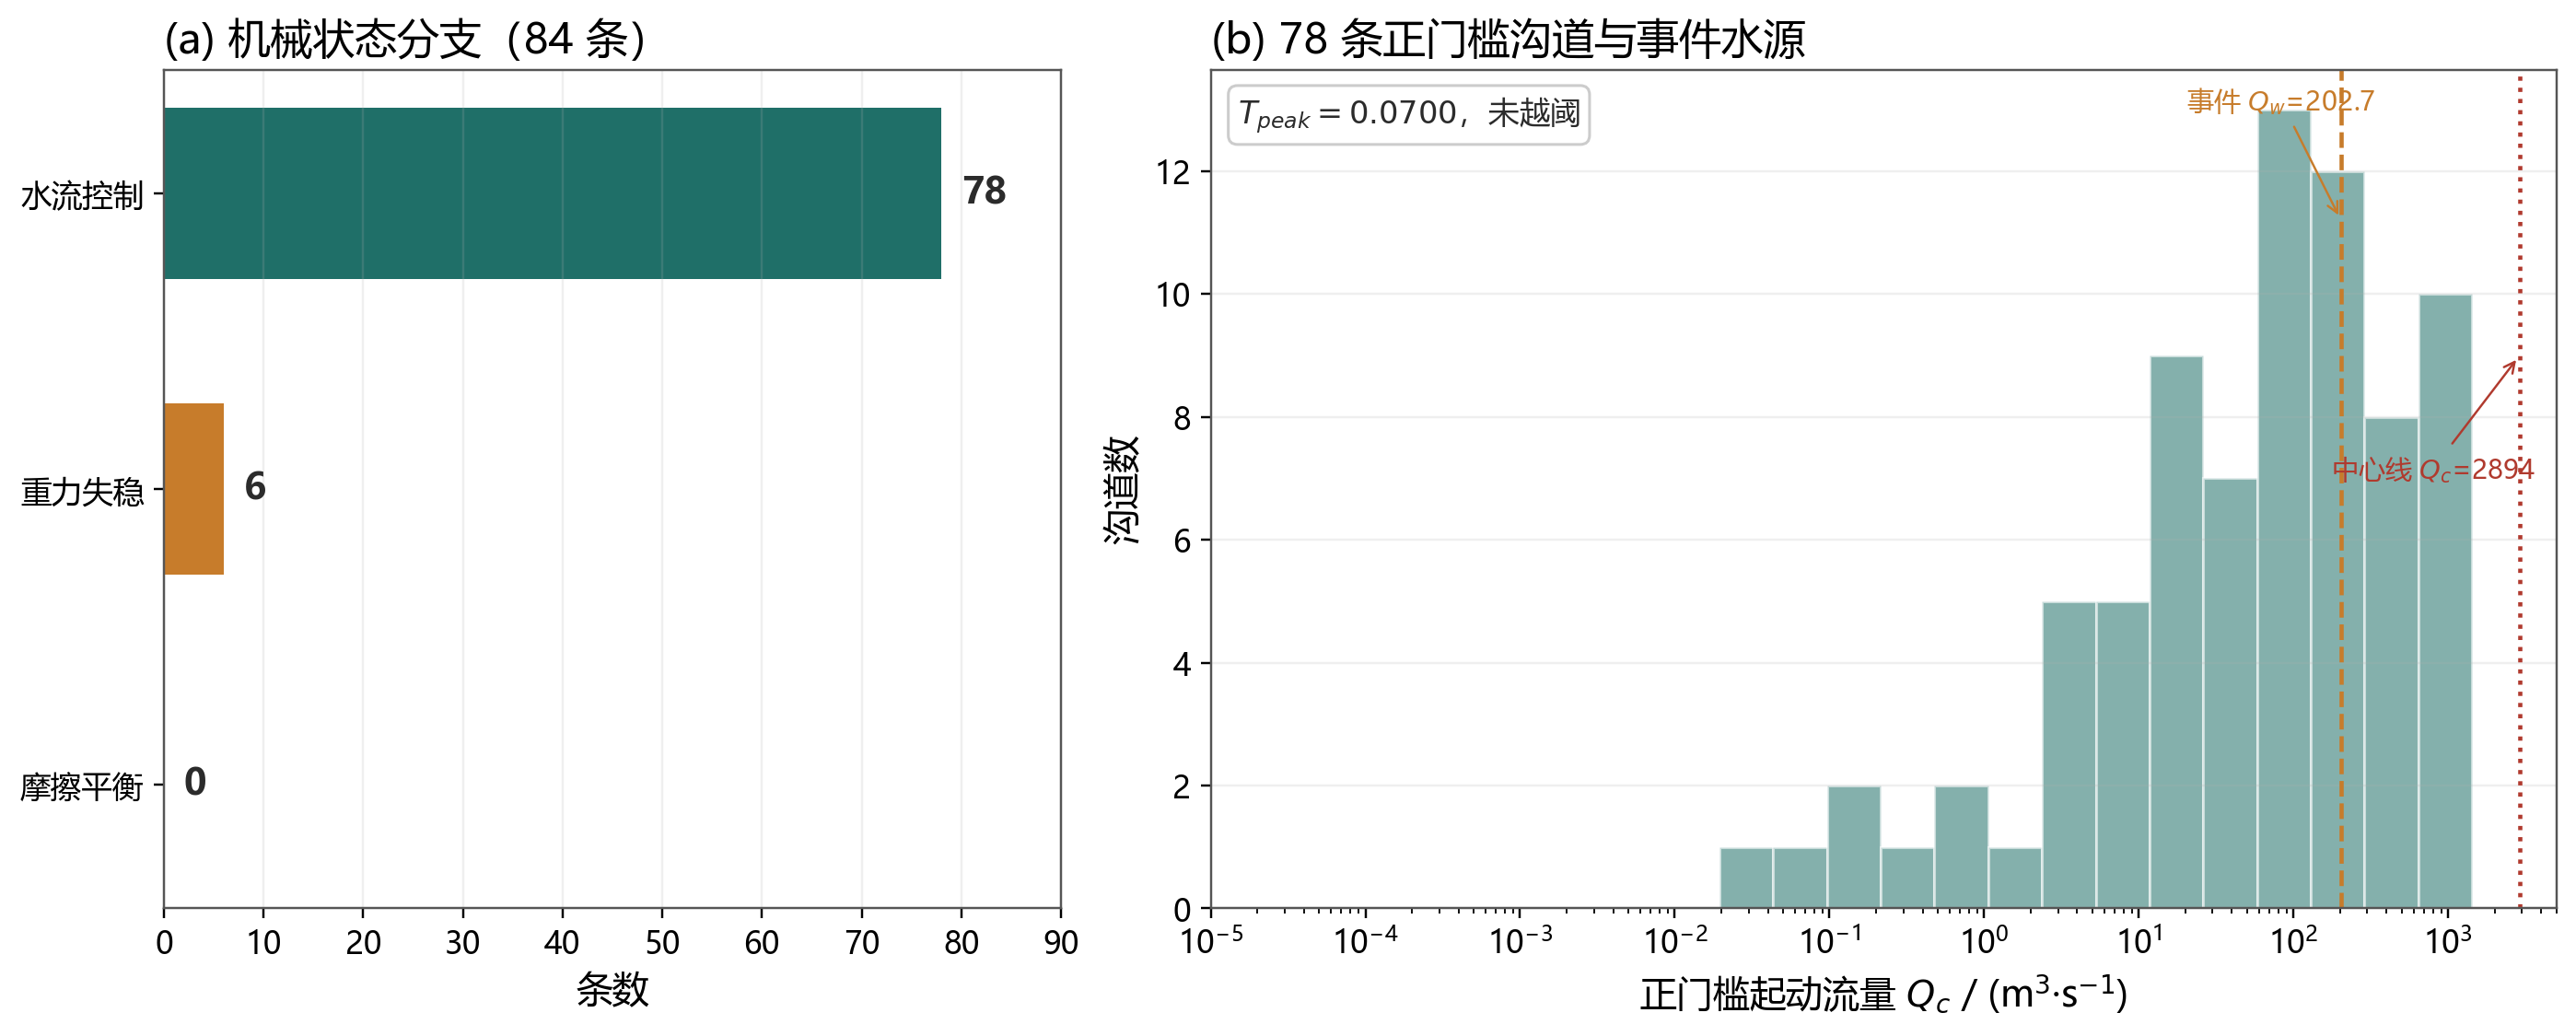
\includegraphics[width=0.92\textwidth]{figures/02_临界条件.png}
\caption{机械状态分支与正门槛流量。左：84条历史沟道的机械状态；右：78条正门槛沟道的$Q_c$分布、事件水源$Q_w$与正式中心线$Q_c$。}
\label{fig:q2-critical}
\end{figure}

\subsection{对象级状态元组与冰崩链状态识别}
84个对象以源数据唯一标识object\_id存储，不使用可重复的显示名称作为主键。每个对象和时刻保存六元组
\begin{equation}
\mathcal R_j=(G_j,H_j,\Theta_j,F_{\mathrm{ice},j},U_{\mathrm{ice},j},C_{\mathrm{ice},j}),
\end{equation}
其中$G$为水流控制、摩擦平衡、重力失稳或不可评估；$H$为水力候选、低于门槛、不适用或不可评估；$\Theta$为热力前兆成立、低于热力参照或不可评估。$F_{\mathrm{ice}}$表示附件4中存在冰厚与坡度同时达到源区阈值的编目像元，本数据中阈值为50 m与25$^\circ$，共335个像元；$U_{\mathrm{ice}}$记录冰体强度、裂隙、位移或监测资料缺失；$C_{\mathrm{ice}}$只在热力前兆成立且$F_{\mathrm{ice}}=1$时为1。

事件时刻将同一口岸集水区水源流量施加于84个历史沟道几何作比较，$H$的计数为44条低于门槛、34条水力候选、6条不适用。该统计是同一流量口径下的条件对照，不是84条沟道在现场同时获得相同水源的观测事实。事件日$\Theta$为低于热力参照，因而对象层$C_{\mathrm{ice}}=0$；但$U_{\mathrm{ice}}=1$表明冰体力学状态仍不可识别，该保留项始终存在。热力未达参考、有限水力比未越1，均不能证明冰体没有失稳，也不能把状态元组压成未经校准的0--1概率。

\subsection{水源流量与事件前处理}
SCS-CN是单场降雨的累计损失模型，初损按完整事件累计，不逐小时重置\cite{hawkins2009}。对完整小时轴，连续六个已观测、严格零降雨小时确认事件边界；短于六小时的干隙保持同一事件，微量正降雨仍属于降雨，不套用I--D筛查的湿小时阈值。设事件起始小时为$s_e$，事件累计雨量为$P_e(t)=\sum_{u=s_e}^{t}P(u)$，累计直接径流曲线与逐时增量为
\begin{equation}
F_e(P)=
\begin{cases}
\dfrac{(P-I_{a,e})^2}{P-I_{a,e}+S_e},&P>I_{a,e},\\[2mm]
0,&P\le I_{a,e},
\end{cases}
\qquad
R_{\mathrm{rain}}(t)=F_e(P_e(t))-F_e(P_e(t-1)),
\label{eq:scs}
\end{equation}
其中$P_e(s_e-1)=0$，$S_e=25400/C_{N,e}-254$，$I_{a,e}=0.2S_e$。单场内初损只扣一次；事件起始前的最后一小时记为$s_e-1$。基准曲线数$C_{N,0}=85$是独立设定的工程情景，不由土地覆盖类码推导。API分位只用2021--2025年6--9月的14640个有效小时计算，固定为$q_1=3.574888$、$q_3=10.194567$；不使用全季节回退，也不用2026年重估。场初曲线数由事件起始前一小时的API确定：
\begin{equation}
C_{N,e}=\operatorname{clip}
\begin{cases}
0.75C_{N,0},&\mathrm{API}(s_e-1)<q_1,\\
C_{N,0},&q_1\le \mathrm{API}(s_e-1)\le q_3,\\
1.15C_{N,0},&\mathrm{API}(s_e-1)>q_3,
\end{cases}
\quad[30,98].
\end{equation}
事件内不再随API改变而重新套用累计公式作差。初始边界、时间缺口或缺测降雨使累计状态未知，须重新观测到六个连续严格零雨小时才恢复已知边界；负雨量和非有限值视为无效，不将负值裁零来制造干期。若场初前一小时API不可用，整个事件的正雨产流记不可评估；已知场初且记录末端未闭合的事件，其已观测前缀仍可计算。汇流继续按原核传播缺测，缺测保持为空。该分级与六小时边界近似前期含水量和事件分隔，缺少本区水文率定；三、六、十二小时边界的函数行为已由单元测试核对。

源区温度由站点温度按0.006 K/m直减率外推至有效冰厚像元平均高程5109.653 m，站点高程取3980 m，温差订正为$-6.7779\ ^\circ$C。融水权重取Logistic温度因子$w_T(t)$\cite{hock2005}，RGI6编目边界与集水区面积交比$f_{gl}=0.23602$。于是
\begin{equation}
m_{\mathrm{src}}(t)=\frac{w_T(t)e_m(t)}{0.334},\qquad
m_{\mathrm{cat}}(t)=f_{gl}m_{\mathrm{src}}(t),
\end{equation}
其中$e_m$以MJ/(m$^2\cdot$h)计，0.334 MJ/m$^2$对应1 mm水当量。雨与融水分别作三小时汇流后，
\begin{equation}
Q_w(t)=\frac{A_{km^2}}{3.6}\left[
\sum_{i=0}^{2}w_iR_{\mathrm{rain}}(t-i)
+\frac13\sum_{i=0}^{2}m_{\mathrm{cat}}(t-i)\right],
\quad
(w_0,w_1,w_2)=(0.6,0.3,0.1).
\label{eq:water}
\end{equation}
$f_{gl}$是编目年代面积权重，不是2026年实时冰雪范围；任一必需小时缺测时，$Q_w$保持缺测。

\subsection{事件窗求解与水力状态}
正式事件窗为2026年8月26日08:00--13:00的六个整点标签。水源窗峰值为202.650179 m$^3$/s，出现在13:00；相对正式中心线门槛，触发比在该时为
\begin{equation}
T_{\mathrm{peak}}=\frac{202.650179}{2.893667\times10^3}
=0.07003232034381977,
\end{equation}
10:00的$T=0.018814$，窗口内$T\ge1$的小时数为0，未出现越阈时刻。该结果说明当前无黏聚、无超孔压水控链条没有把此次冰崩链识别为水力越阈事件；它不说明冰体未失稳，反而要求保留$U_{\mathrm{ice}}=1$的冰力学未识别状态。旧事件窗标定系数$k=11.19431$仅作对照，正式模型不使用事件窗$k$，也不将窗口水源峰值归一为1。

\begin{figure}[htbp]\centering
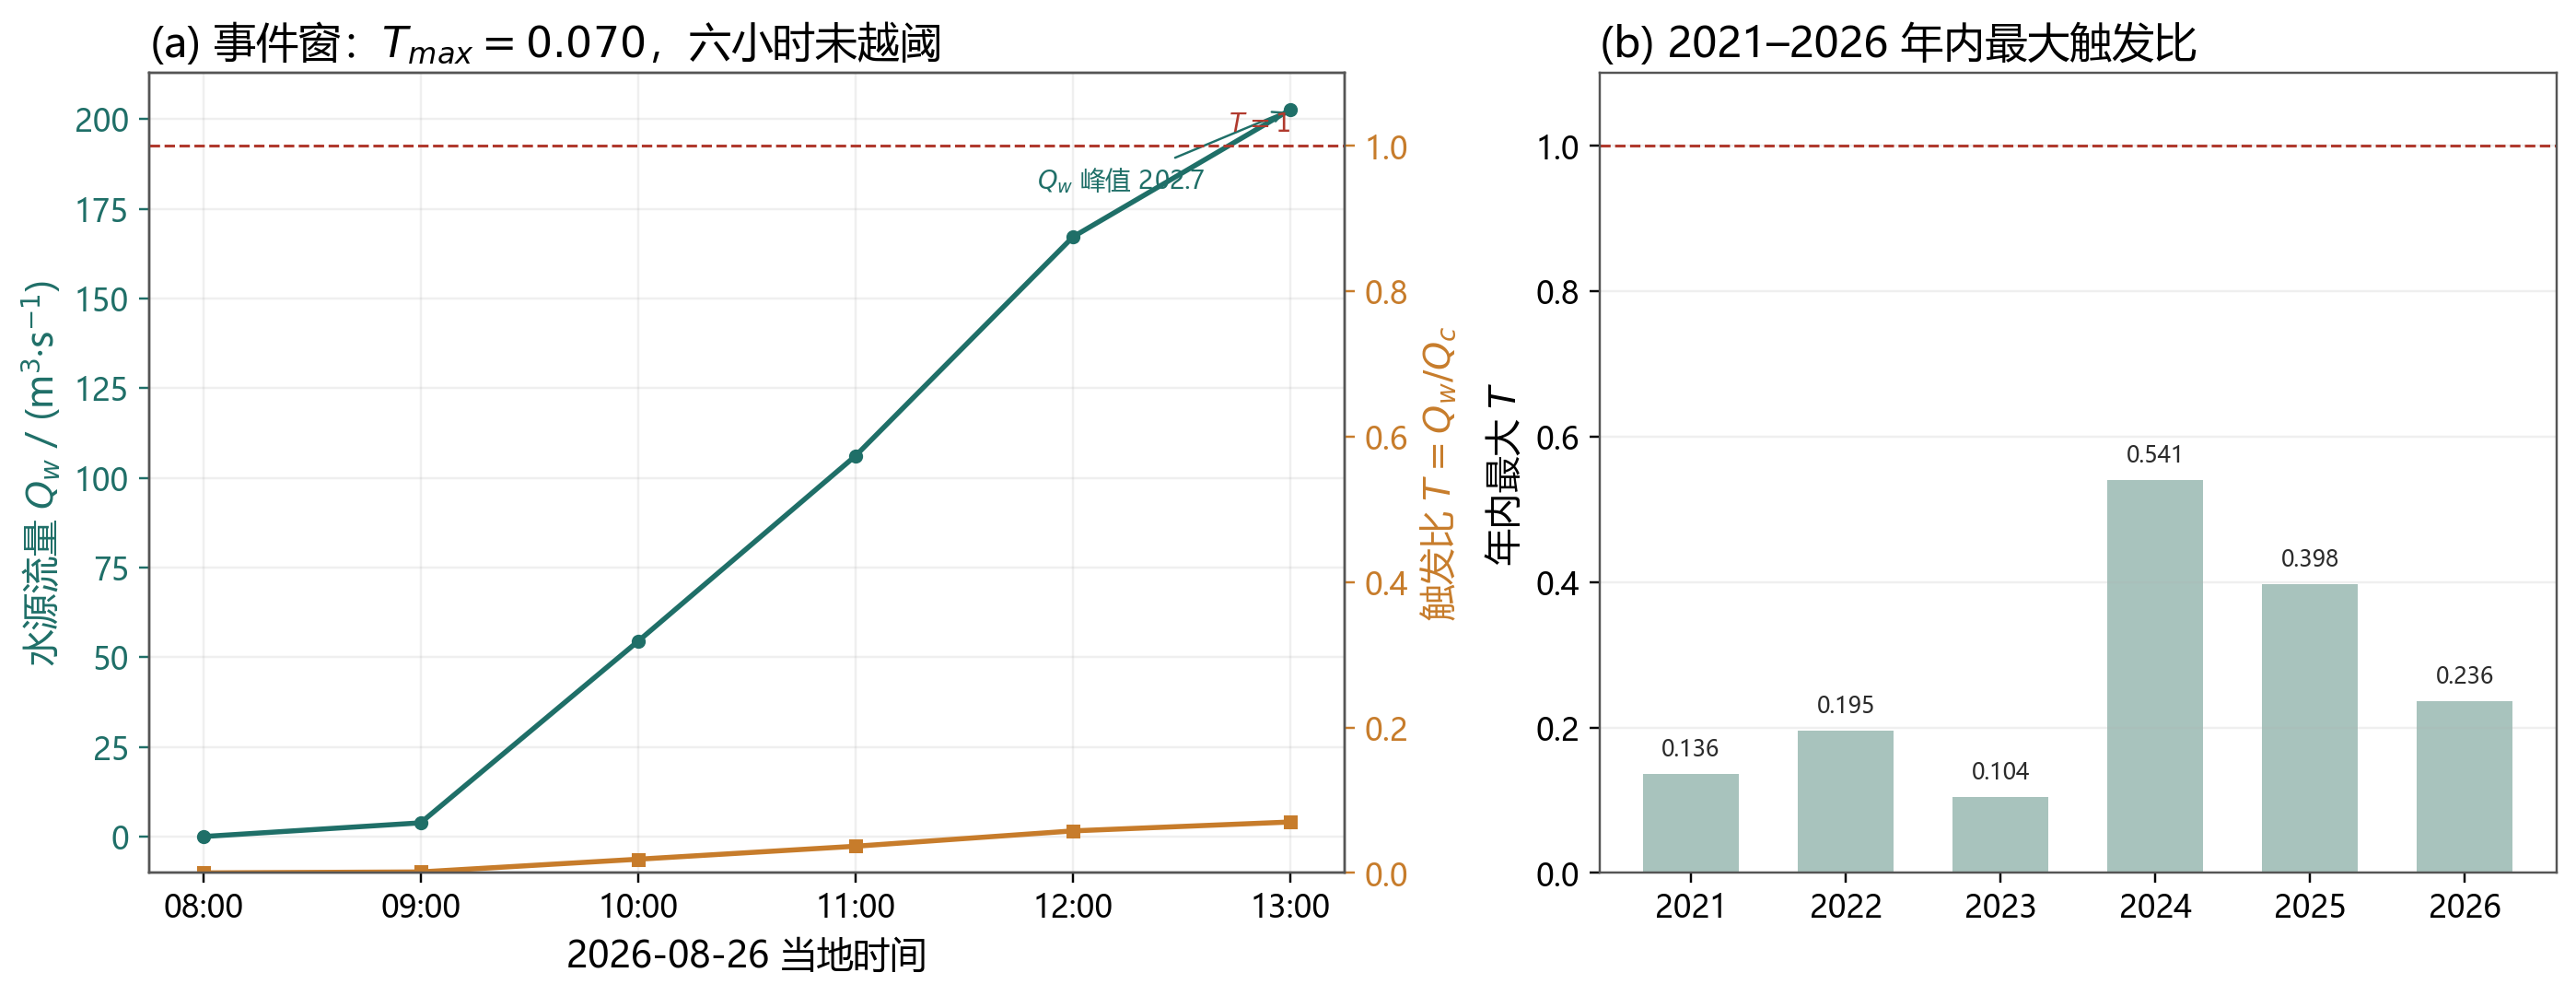
\includegraphics[width=0.94\textwidth]{figures/02_触发评估.png}
\caption{事件窗水源与触发比。(a) 2026-08-26 08:00--13:00；(b) 2021--2026年最大触发比。}
\label{fig:q2-trigger}
\end{figure}

图\ref{fig:q2-trigger}把事件窗与年内最大触发比放在同一条件门槛下展示；图中$T$是条件强度比，不是发生概率，事件窗内未出现$T\ge1$。未越阈是当前模型的结果，不是对冰体失稳或链式过程发生的否定。

\subsection{历史规模关联与双语义降雨包络}
在78条水流控制正门槛对象上，分别检验总起动流量$Q_{\mathrm{crit}}=q_{\mathrm{crit}}B/\kappa_B$和单宽起动流量$q_{\mathrm{crit}}$与已发生对象规模排序的关系，二者名称与量纲需分开。总流量对规模的Kendall检验为$\tau=0.408386$、$p=5.471436410144295\times10^{-6}$，Spearman检验为$\rho=0.498676$、$p=3.3745699520687622\times10^{-6}$；单宽流量对规模的Kendall检验为$\tau=0.318602$、$p=3.904720246143714\times10^{-4}$，Spearman检验为$\rho=0.400620$、$p=2.784782801479891\times10^{-4}$。四组$p$值均按双精度和科学计数法保留，不静默舍入为零。正相关表明在本已发生对象中，较大规模沟道并不具有更低的流量门槛；它不支持发生概率方向，也不能外推到未发生沟道。

降雨阈值保持两种语义\cite{guzzetti2008}。138场完整降雨过程给出的95\%频率包络为$I_{95}(D)=6.3507D^{-0.5853}$，事件平均强度的10\%分位参考为$I_{10}(D)=1.0000D^{-0.7374}$，$D$以小时计、$I$以mm/h计。前者描述历史稀有度，后者只是未作灾害标注的低分位候选筛查线；二者含义不同，不取平均；“超过包络”只表示历史稀有，不表示真实起动。完整样本支持到12小时，更长时间的幂律仅作外推提示。两条线的位置对照见图\ref{fig:q2-id}。

\begin{figure}[htbp]\centering
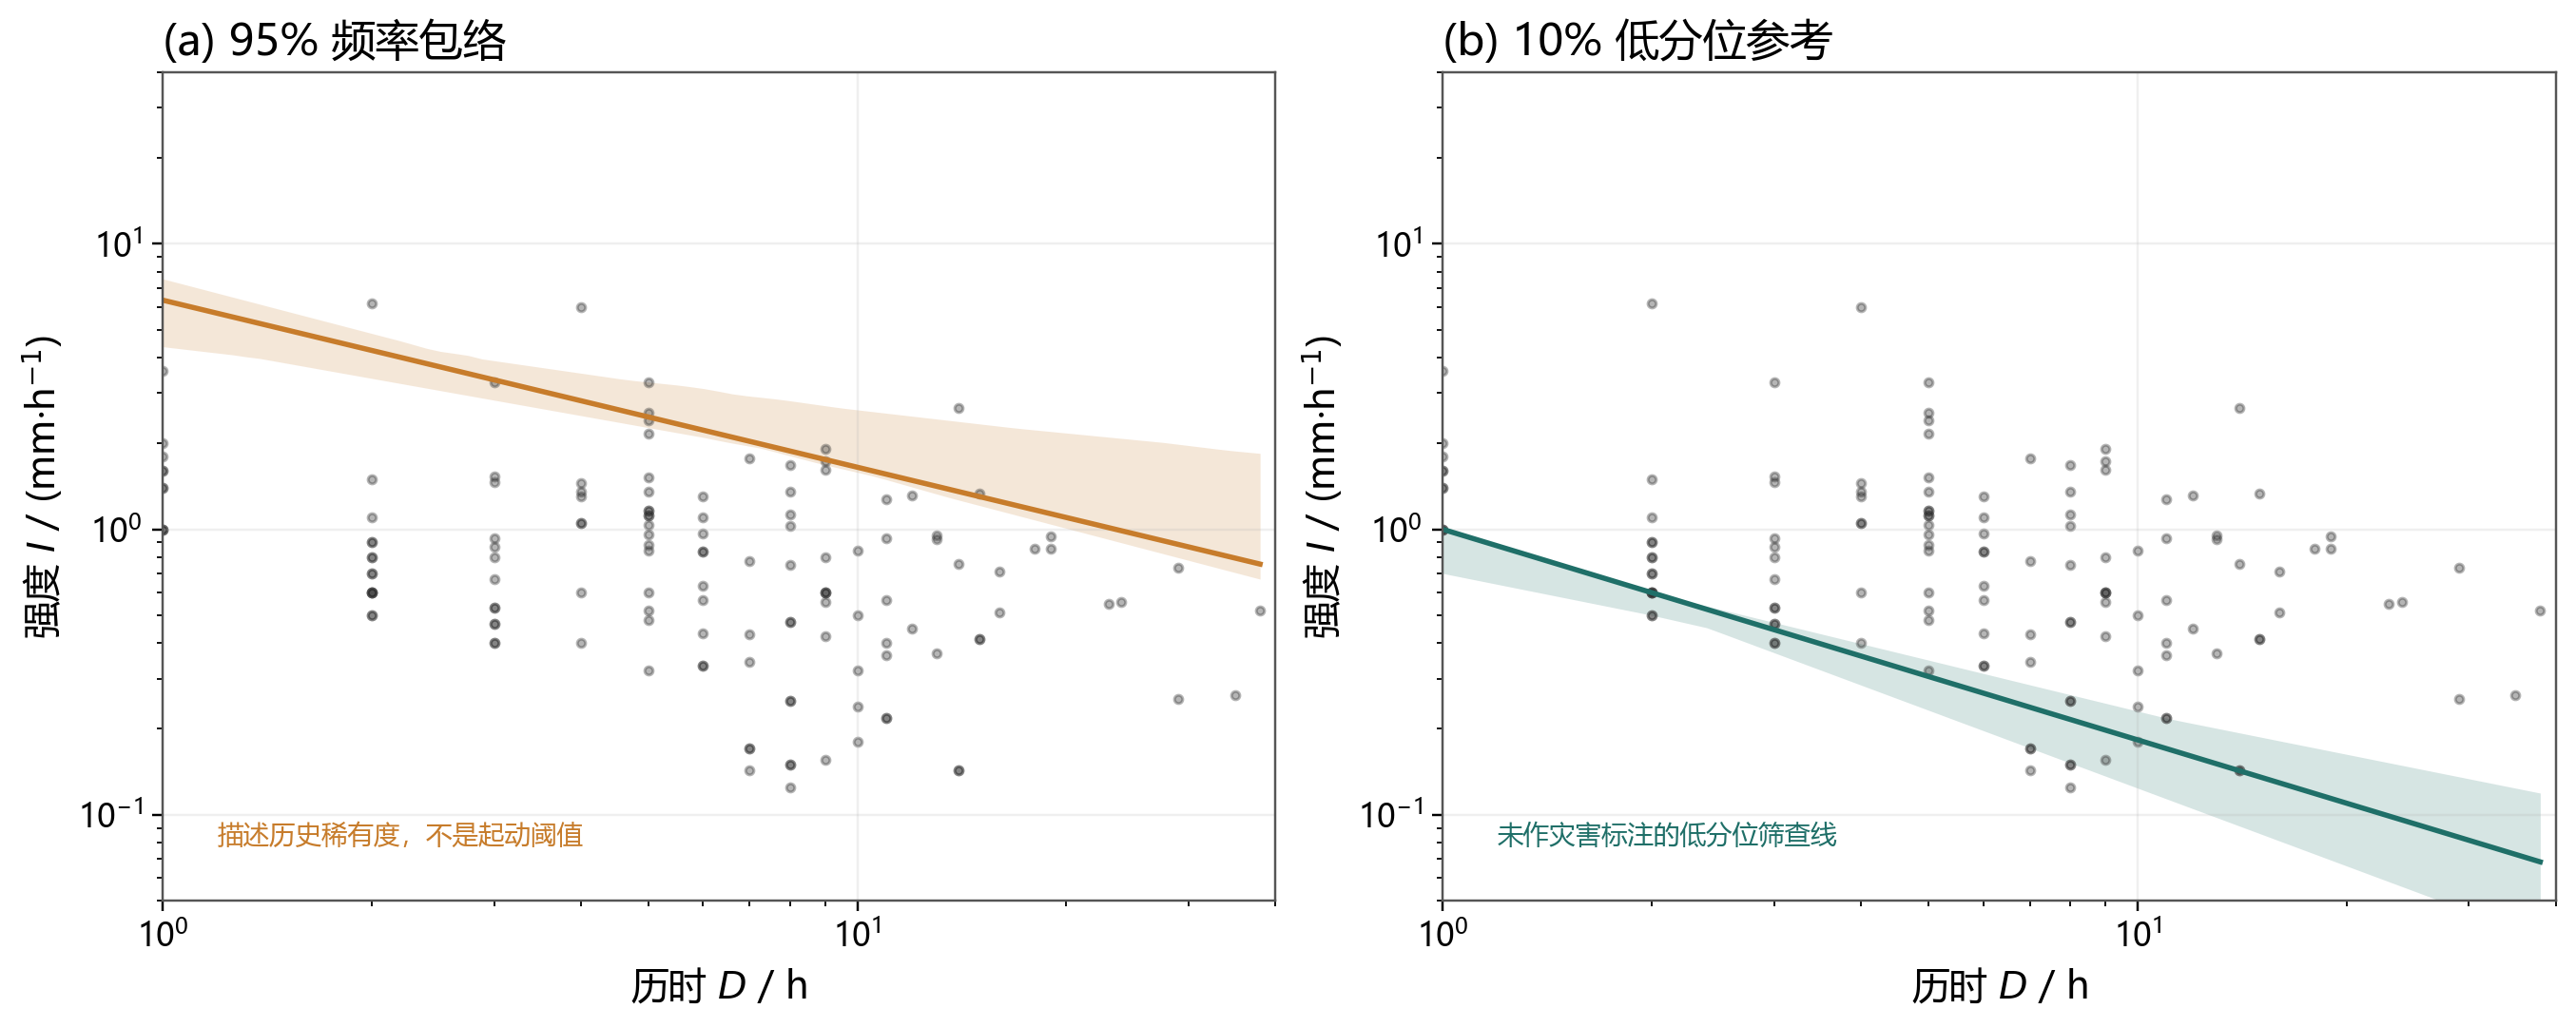
\includegraphics[width=0.92\textwidth]{figures/02_I-D包络.png}
\caption{两种降雨阈值语义。(a) 95\%频率包络；(b) 10\%低分位参考。灰点为完整降雨过程样本。}
\label{fig:q2-id}
\end{figure}

\subsection{时间与空间可靠性}
时间聚合按同一有效窗比较。3、6小时和日尺度的有效窗口数分别为10583、4980、1190，平均/峰值保持率为0.722655、0.537989、0.230808；三种聚合下均无$T\ge1$窗口。2021--2026年最大$T$分别为0.136392、0.195132、0.104129、0.540807、0.397600、0.235953，均明显低于1。全序列触发评分$P$的最大值为0.137433，出现在2024-09-28 18:00，也远低于0.5的报文门槛。平均会削弱短脉冲，但本数据中即使取窗内峰值也未越阈；该负值反映当前参数与分辨率下的模型行为，不表示现场未发生链式过程。

继承像元对照在30、90、270米名义尺度上的LR AUC分别为0.9814、0.9269、0.8790，组块自举区间分别约为$[0.9757,0.9872]$、$[0.8984,0.9571]$、$[0.8355,0.9195]$。这些数值主要反映灾点面内正像元与面外500米背景的采样环境差异；背景没有确证非灾真值，不代表发生概率或危险区划。共同候选域统一DEM、覆被、最小地面面积和500米隔离后，三尺度均只形成2个正组和188个背景组，无法形成至少两折同时含两类的训练/测试划分，因此不报告AUC。图\ref{fig:q2-common-domain}展示共同域、物理块和空间隔离的诊断结果。

\begin{figure}[htbp]\centering
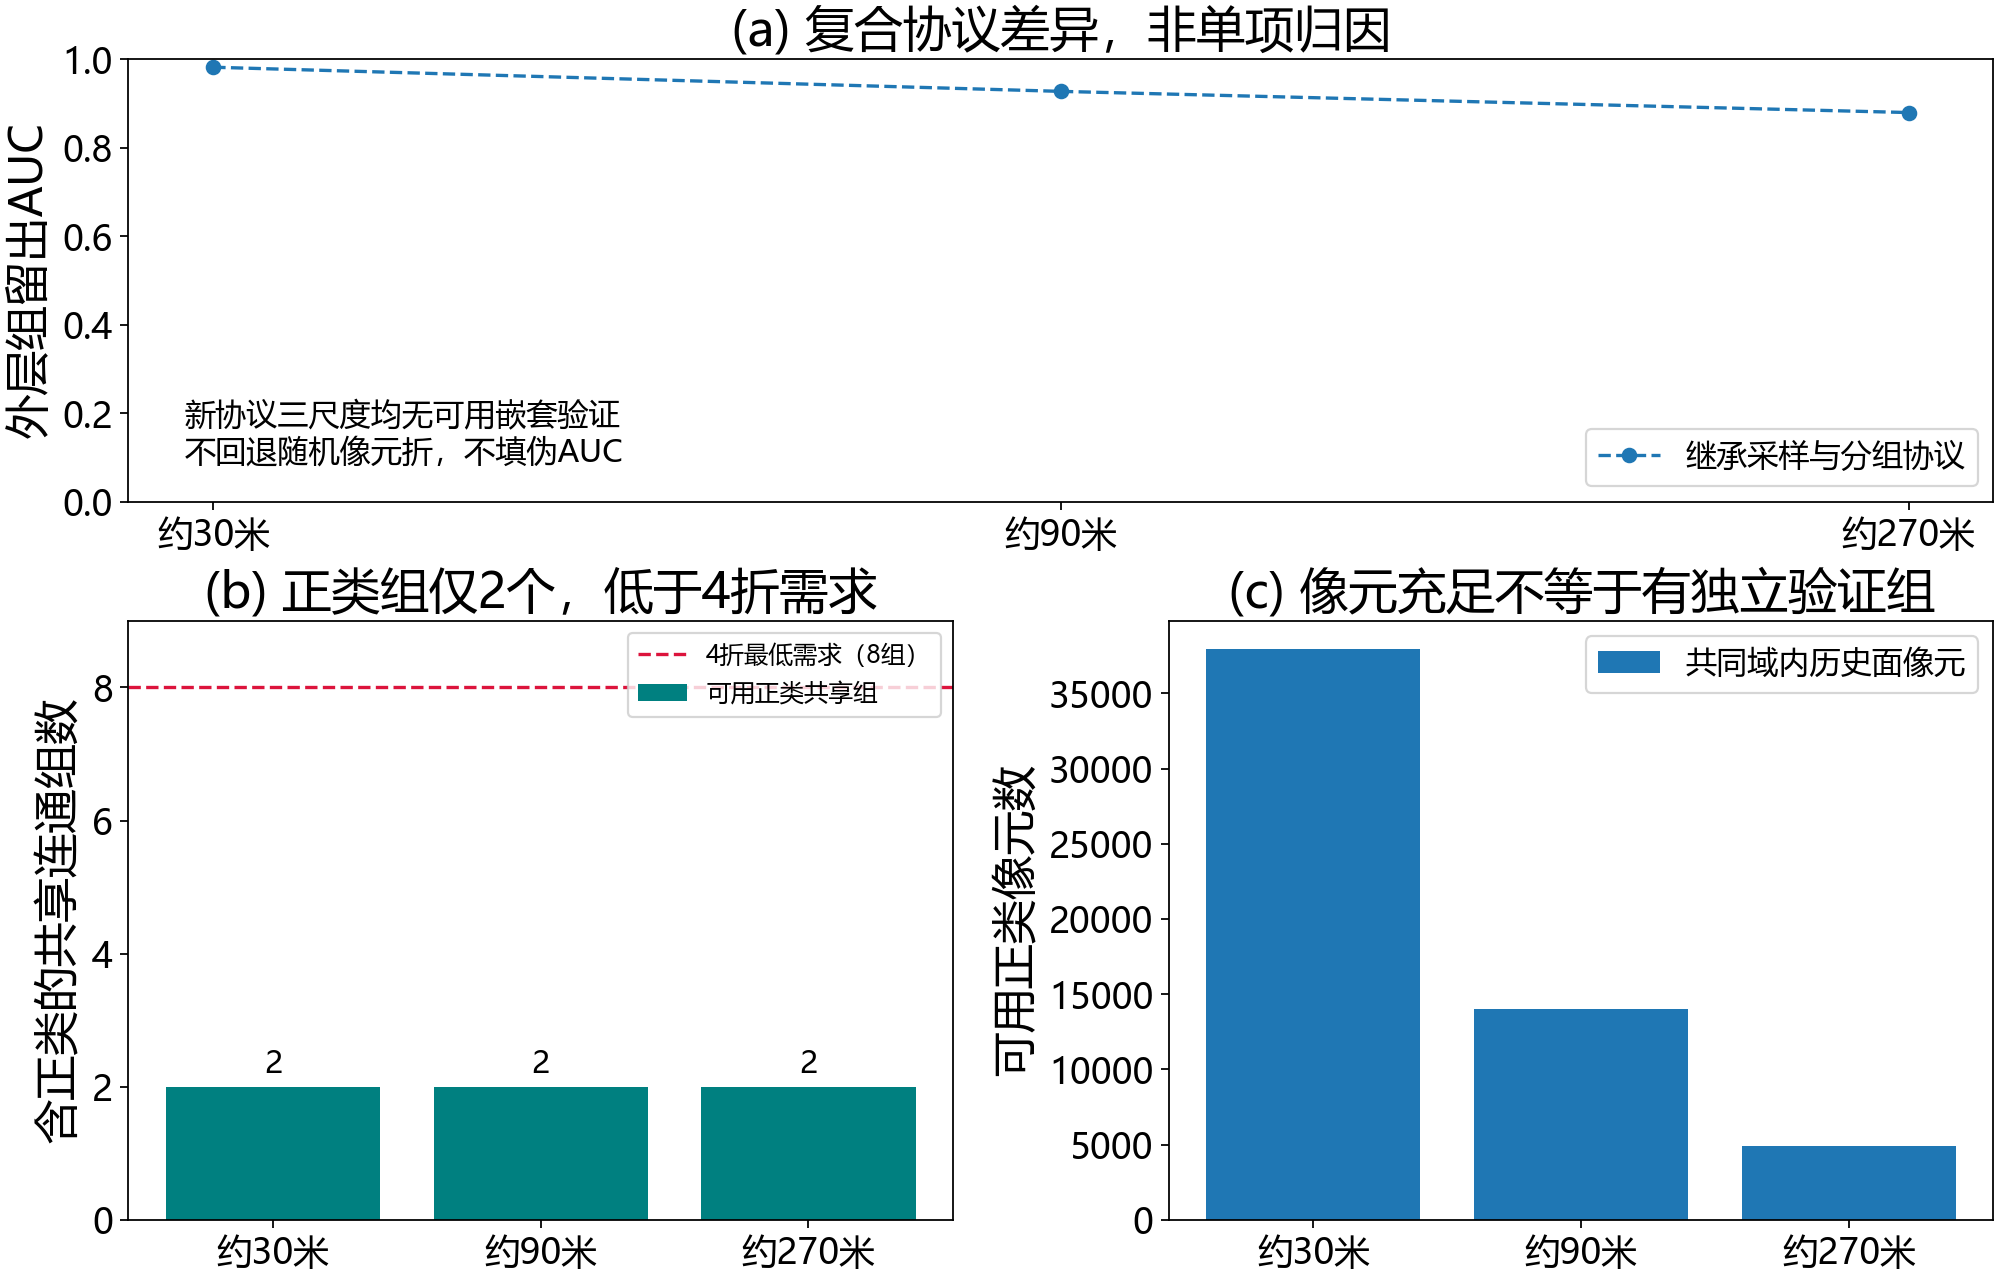
\includegraphics[width=0.92\textwidth]{figures/02c_共同域空间隔离.png}
\caption{共同域空间隔离诊断}
\label{fig:q2-common-domain}
\end{figure}

分辨率和路径口径也会改变门槛。用于D8追迹敏感性检验的主沟比降在2--6倍粗化下为0.084354--0.086502，单宽临界流量约86.699--89.999 m$^2$/s，集水区面积相对偏差绝对值不超过0.4814\%，但口岸投影偏移最大约83.4 m。上述范围与正式中心线门槛不混作同一口径：前者检验路由和粗化稳定性，后者使用公共注入至口岸中心线。中心线平均比降不覆盖每个局部起动段；跨尺度移植时宽度、汇流和床面材料可能同时变化。

\subsection{综合判读}
正式链条是“床体沿坡自重＋水流拖曳与大有效法向摩擦”的条件力平衡，再经$h_c$、$q_c$、Manning和$Q_c$转换到断面尺度。84条历史沟道中78条仍需正水流门槛、6条在给定模型参数下重力失稳。事件窗中心线水源峰值202.650179 m$^3$/s对应$T_{\max}=0.070032$，10:00仅0.018814，当前水控模型未越阈；冰体源区虽有335个达到50 m/25$^\circ$阈值的像元，但强度、裂隙和位移资料缺失，冰力学状态仍未识别。空间上仅能确认继承采样环境的可分性，严格共同域因正组不足而不可估计；时间上仅能确认水控门槛未越，而水控未越不等于冰崩链未发生。模型适用于有有效几何且床面假设落在给定范围内的条件评估；真实发生概率、无资料沟道安全认证和未经校准的危险区划不在本文范围。

\section{问题三：固定发布时刻的条件预报与真实触发识别}
\noindent\textbf{本问结论：}固定08:00发布，源区融水起始代理$t_m$的条件区间为09:03:22--10:57:51，即时释放条件到达$t_a^{(0)}$为09:35:26--11:31:59；10:30仅落入辅助区间（1/1），不代表真实覆盖。真实释放$t_r$、形成$t_f$、实际到达$t_a$、真实预警与覆盖率均不可估计。

\subsection{任务目标与可识别范围}
题目要求给出触发时间的95\%置信区间、预警时间、区间覆盖率和空间距离。现有资料只有一个口岸冲击时刻，没有源区冰体失稳、物料释放或泥石流形成的独立时间观测；附件4的表面速度是2014--2024气候态栅格，没有2026年灾前时间维。因而现有资料不足以识别真实释放时刻$t_r$、形成时刻$t_f$、实际到达$t_a$及其预警和覆盖率。

本文把时间对象分开。$t_m$为源区融水条件首次满足的代理时刻，$t_a^{(0)}$为“融水出现即释放既定物料”情景下的口岸条件到达，$t_a$为实际到达。三者满足
\begin{equation}
t_r\ne t_m,\qquad
t_f=t_r+\Delta_{r\to f},\qquad
t_a=t_r+\Delta_{r\to\mathrm{inj}}+\Delta_{\mathrm{inj}\to a},
\label{eq:times}
\end{equation}
其中$\Delta_{r\to f}$为释放到流态转变的延迟，$\Delta_{r\to\mathrm{inj}}$为释放到公共注入断面的传播时间，$\Delta_{\mathrm{inj}\to a}$为注入到口岸的运行时间。没有释放观测时，本文不把$t_m$当作$t_r$，也不把$t_a^{(0)}$写成实际到达。表\ref{tab:q3-targets}列出各目标的处理。

\begin{table}[htbp]\centering\footnotesize
\caption{第三问目标与可识别性}\label{tab:q3-targets}
\begin{tabular}{@{}l l l@{}}\toprule
目标&可识别性&本文输出\\\midrule
$t_m$：源区融水起始代理&辅助气象目标&条件95\%区间\\
$t_r$：冰岩物料实际释放&不可识别&空值\\
$t_f$：泥石流形成&不可识别&空值\\
$t_a$：口岸实际到达&不可识别&空值\\
$t_a^{(0)}$：即时释放条件到达&辅助情景&条件95\%区间\\
10:30口岸冲击&题面单一锚点&事后单点包含\\
\bottomrule
\end{tabular}\end{table}

因此，本文给出的产品是$t_m$与$t_a^{(0)}$的条件区间、状态计数和空间距离。真实$t_r$、$t_f$、$t_a$、真实预警和覆盖率尚不能给出；当前结果属于辅助条件产品，不作为真实触发预报。

主发布时刻固定为2026年8月26日08:00当地时（00 UTC），预报窗口为
\begin{equation}
\mathcal H=[2026\text{-}08\text{-}26\,08{:}00,\,
2026\text{-}08\text{-}27\,08{:}00).
\end{equation}
主起报为8月25日18 UTC，另取同日06、12 UTC两次单次起报构造模式演化差异。三者按六小时分发上界分别于25日12 UTC、18 UTC和26日00 UTC可用，均不晚于发布时刻；每次起报生成1000个成员，合计$N=3000$。题面10:30只用于事后单点包含，不进入成员生成、系数拟合或配置选择。

\subsection{变量时间对齐与历史能量关系}
普通小时短波是前一小时均值，降水是前一小时累计，温湿度是对应时点的瞬时值。若按原始标签把三者放在同一行，会把前一小时间接辐射归入后一小时支持。本文按变量真实支持对齐到统一半开区间$[t,t+1)$：
\begin{equation}
SW_t=SW^{\mathrm{raw}}_{t+1},\qquad
P_t=P^{\mathrm{raw}}_{t+1},\qquad
\bar T_t=\frac{T^{\mathrm{raw}}_{t}+T^{\mathrm{raw}}_{t+1}}{2},\qquad
\overline{RH}_t=\frac{RH^{\mathrm{raw}}_{t}+RH^{\mathrm{raw}}_{t+1}}{2}.
\label{eq:support}
\end{equation}
前两者是过去小时均值与累计量，后两者是时点值的梯形均值近似。先取小时均值，再施加正部与门控，不交换非线性操作；任一端点缺失则该小时不可评估，不用下一条记录跨过时间缺口。发布前最后完成支持$[07{:}00,08{:}00)$取原始标签08:00的短波与降水，以及两个温湿端点；完整轨迹的末支持起点为原始末时点减一小时。若按起始标签对齐，会把前一小时间接辐射归入后一小时支持，故本文不采用该口径。

历史站点四类小时标签缺少起止或瞬时元数据。主假设为MET时点端点梯形均值、RADM/SOIL/FLUX起点标签小时均值；对MET三种处理与其余三族起点/终点组合共24种情形重建净辐射与消融能量目标、重拟合回归和AR(1)，各情形使用同一流程，未按事件结果挑选。24种情形给出相同的成员首达支持集合，说明辅助区间对时间标签假设不敏感；真实释放仍需独立观测。

在2021--2025年6--9月共同有效小时上拟合
\begin{equation}
\hat e_m=\beta_0+\beta_T T^++\beta_R R^++\beta_H RH+\varepsilon,
\qquad
T^+=\max(T,0),\quad R^+=\max(SW,0),
\end{equation}
其中$\hat e_m$与$R^+$的单位为W/m$^2$，$T$为$^\circ$C，$RH$为百分数。训练集共11986行，估计得
\begin{equation}
\beta=(-119.0252,\,-5.8526,\,0.4706,\,1.7154),
\end{equation}
残差一阶自回归参数$\phi=0.400328$、创新标准差$\sigma_\varepsilon=41.015695$ W/m$^2$，边际标准差44.715577 W/m$^2$，连续小时对11772个。预报时仅当$T>0$、$SW>20$ W/m$^2$且$\hat e_m>0$时判定潜在融水；任一必需输入缺失记不可评估，不以零值填补。小时水当量按$m_s=\hat e_m/334000\times3600$换算。

发布前最后完成支持$[07{:}00,08{:}00)$没有成员满足活动判据。发布后24小时窗内，3000个源区成员和3000个传播成员均判定为有效，有效比例$p_{\mathrm{fin}}=1$；无事件、发布时已活跃、右删失、不可评估、未到达及口岸左删失的成员计数均为0，状态合计一致。可行动质量
\begin{equation}
p_{\mathrm{actionable}}=p_{\mathrm{act}}+p_{\mathrm{fin}}=0+1=1
\end{equation}
只表示给定模型集合中需要发出源区融水提示的成员比例，不是物理发生概率。

\subsection{条件区间与支持包络}
每个成员的小时支持原样保留为$[L_i,U_i)$，宽度为1 h。为给出事件时刻分位，在固定随机流中为每个有限成员在支持内均匀抽取代表时刻
\begin{equation}
\tilde t_i=L_i+\tau_i(U_i-L_i),\qquad \tau_i\sim U[0,1),
\end{equation}
再取2.5\%与97.5\%分位。$t_m$与$t_a^{(0)}$由同一成员、同一传播配置配对生成：
\begin{equation}
\tilde t_{a,i}^{(0)}=\tilde t_{m,i}+\Delta t_{\mathrm{fall},i}
+\Delta t_{\mathrm{run}}^{(c_i)},
\end{equation}
其中$\Delta t_{\mathrm{fall}}$为源区质心至公共注入断面的无摩擦首波近似，两种高程语义下为29.50--29.67 s；$\Delta t_{\mathrm{run}}^{(c_i)}$取自16个去重D8配置之一。配置等权抽样只表示模型集合设计，不是现实配置概率。

条件区间见表\ref{tab:q3-event-intervals}，均为2026年8月26日UTC+8时刻，保留到毫秒。它们是有限成员分布内的名义95\%分位，不是经真实多事件频率校准的信赖区间。

\begin{table}[htbp]\centering\footnotesize
\caption{条件事件时刻区间}\label{tab:q3-event-intervals}
\begin{tabular}{@{}l c c c c@{}}\toprule
对象&2.5\%分位&中位&97.5\%分位&宽度/h\\\midrule
源区$t_m$&09:03:22.847&10:13:44.990&10:57:51.047&1.907833\\
即时释放$t_a^{(0)}$&09:35:26.068&10:46:31.992&11:31:59.410&1.942595\\
\bottomrule
\end{tabular}\end{table}

完整支持包络与支持端点分位不是同一对象。前者为有限成员全部半开支持的凸包
\begin{equation}
E_{\mathrm{support}}=[\min_i L_i,\max_i U_i),
\end{equation}
可能含空档，不是成员支持的精确保集；后者为
\begin{equation}
E_{0.95,\mathrm{endpoint}}=[q_{0.025}(L_i),q_{0.975}(U_i)],
\end{equation}
只是端点边际分位的收缩诊断。两者均不替代表\ref{tab:q3-event-intervals}的代表时刻事件区间，具体数值见表\ref{tab:q3-envelopes}。

\begin{table}[htbp]\centering\footnotesize
\caption{支持包络}\label{tab:q3-envelopes}
\begin{tabular}{@{}l c c c c@{}}\toprule
对象&包络类型&起点&终点&宽度/h\\\midrule
$t_m$&完整支持&$[$09:00:00.000&11:00:00.000$)$&2.000000\\
$t_m$&端点2.5\%/97.5\%&$[$09:00:00.000&11:00:00.000$]$&2.000000\\
$t_a^{(0)}$&完整支持&$[$09:18:03.728&11:45:13.334$)$&2.452668\\
$t_a^{(0)}$&端点2.5\%/97.5\%&$[$09:26:42.679&11:45:13.170$]$&2.308470\\
\bottomrule
\end{tabular}\end{table}

三类时间对象的分工见图\ref{fig:q3-time-products}；图中深条为代表时刻的2.5\%--97.5\%条件区间，浅条为完整支持包络，底部灰条明确标出真实$t_r$、$t_f$、$t_a$不可识别，不把不同定义混成一个“95\%触发区间”。

\paperfig{figures/03_时间区间.png}{0.96}{条件区间、支持包络与10:30口岸锚点。灰色行为不可识别时刻}{fig:q3-time-products}

\subsection{单事件包含、提示时差与真实预警}
真实泥石流形成没有独立真值，真实触发覆盖率不可估计，本文不给出数值。题面只给出一个口岸冲击点$y_h=10{:}30$。在即时释放辅助情景下，条件区间09:35:26.068至11:31:59.410包含该点，报告为1/1。该1/1表明辅助情景与题面锚点不矛盾，不代表实际到达覆盖率。实际到达覆盖记为不可估计（释放模型未识别），区间、确定覆盖和可能覆盖尚未给出；长期频率需独立资料。

融水提示规则在发布时刻确定：若$p_{\mathrm{actionable}}\ge0.5$，则在08:00发布源区融水提示。本次$p_{\mathrm{actionable}}=1$，故提示时刻为08:00。相对10:30锚点的信息时差为2.5 h，这是“融水提示”相对既有冲击锚点的时间差，不是真实灾害预警提前量。真实灾害预警的首次报警、可执行报警和提前量尚不能给出。

辅助到达区间相对10:30的提前量为
\begin{equation}
\Delta_{a,\mathrm{range}}
=[10{:}30-U_{t_a^{(0)}},\,10{:}30-L_{t_a^{(0)}}]
=[-1.033169,\,+0.909426]\ \mathrm{h},
\end{equation}
区间跨过锚点，故2.5 h信息时差不构成命中提前量；源区代理中位距发布2.229 h，也不是真实释放提前量。图\ref{fig:q3-coverage}给出辅助单点包含和提示延迟对照；真实释放、形成、实际到达和真实灾害预警均标注为不可估计。

\paperfig{figures/03_区间覆盖率.png}{0.78}{辅助单点包含与提示时差}{fig:q3-coverage}

\subsection{空间距离与右删失运程}
按同一源区、公共注入断面和口岸代理断面分别计算距离。源区至注入断面的水平距离为2041.449 m；注入断面至口岸代理的中心线沿沟距离为20882.237 m；组合沿沟路线为22923.686 m。源区至口岸代理的平面直线距离为14771.715 m。沿沟里程与平面直线距离不可相加成一个“距离范围”。

16个去重D8配置的口岸首达时间范围为1054.226--2683.668 s，即17.57--44.73 min。全部配置的终态分析域里程均为26045.494670 m，且右删失标志为真；该值是演算分析域末端的右删失前缘，不是自然最大运程，也不是实测危险区边界。空间对象与状态见图\ref{fig:q3-distance}。

\paperfig{figures/03_空间距离.png}{0.80}{沿沟距离与D8到达}{fig:q3-distance}

\subsection{真实释放的识别条件}
式\eqref{eq:times}中的$t_r$不能由融水代理替代。可检验的观测约束路径是渐进破坏的逆速度模型。若取得发布前各时点$u_j$的独立位移$d_j$、相关误差与可用时刻，则对加速段构造
\begin{equation}
v_j=\frac{d_j-d_{j-1}}{u_j-u_{j-1}},\qquad
\dot v=A v^\alpha,
\end{equation}
当$\alpha=2$时
\begin{equation}
v^{-1}(u)=a+bu,\qquad t_r=-a/b\quad(b<0).
\end{equation}
它把可观测加速连接到渐进破坏的预测外推，但仍需检验稳定运动基线、窗口敏感性、测量误差、速度求差相关性和外推失效。附件4的速度场没有2026年时间维，无法构造$v_j(u_j)$；一张气候态速度图或空间四分位带也无法给出$a,b,\alpha$或释放时间区间。用10:30口岸冲击反推$a,b$属于事后标定，本文不采用。

在取得合格序列前，释放状态记为“未知”，不记为“未释放”；真实$t_r$、$\Delta_{r\to f}$、$t_a$及其预警尚不能估计。所需资料包括：发布前源区位移、裂隙开度、地震或声学释放信号，可核查的释放时刻和泥石流形成时刻，以及测量误差与缺测记录。取得这些资料后，才能把真实触发区间、真实预警和独立覆盖率作为主产品重新计算；本文不将当前结果表述为真实触发预报。

\subsection{一致性检查与适用限制}
本节的一致性检查包括：成员总数为3000，源区与口岸状态合计均为3000，支持宽度均为1 h，$p_{\mathrm{actionable}}$与状态质量一致，16个D8配置均提供有限首达，24种站点小时支持组合给出相同辅助区间。这些检查说明成员生成、支持传播和状态记录一致；融水代理不等同于真实释放或泥石流形成，区间也不具备真实频率覆盖。

主要不确定性如下。第一，IFS格点温度、短波和湿度是模式输出，跨高程与地表类型迁移可能产生系统偏差。第二，残差自回归、回归系数扰动和D8配置抽样组成模型集合不确定性，各分量未由多事件联合校准。第三，D8配置等权不是物理概率，改变配置集合会改变条件分位。第四，附件4速度场是气候态，只提供长期背景，缺少灾前加速序列；释放机制仍不可识别。第五，题面仅有一个口岸冲击时刻，无法检验长期覆盖率或误报率。因此，本节给出固定时刻的条件辅助产品及其适用范围，不将单事件结果升级为真实灾害确定性预测。

\section{问题四：双引擎情景演算、右删失处理与有限库存机制}
\noindent\textbf{本问结论：}链A混合入沟体积$2.635835\times10^6$ m$^3$；D8基线32.766603 min到达口岸代理，16个配置全部在26045.494670 m分析域末端右删失；一维基线在9.336769 km自然停止，未到口岸。质量相对残差$2.075820\times10^{-15}$只说明离散记账闭合，不构成地形、流变或现场过程验证。

\subsection{任务目标与模型定位}
问题四要求在给定灾前地形、源区体积与传播参数下，估计过程沿沟演进、口岸到达时间、运程和影响强度。现有资料缺少真实释放过程、沿程侵蚀物源、实测流深流速和现场流变，故本文建立参数透明的条件情景模型，而不把结果称为已率定的灾害重建。两个引擎承担不同任务：一维纵剖面用于检验准恒定断面下的自然停止与沿程尺度；D8网络用于显式连续性推进，输出首达场、历史峰值、终态场和质量收支。D8每格只向一个下游格路由，不含横向动量、漫滩扩散和完整浅水方程\cite{obrien1993}。

两个引擎使用同一公共注入断面和同一口岸代理断面，并以注入断面统一计时。口岸代理是题面地点在DEM上的吸附断面，不是实测受灾断面；全域出口是另一对象，不能代替口岸断面。两引擎结果差异用于揭示结构不确定性，不是两次独立观测，也不因D8到达口岸而删除一维自然停止的结果。

\subsection{公共几何、源区体积与注入边界}
在附件4原生冰川网格上，以冰厚至少50 m且坡度至少25$^\circ$筛选源区，共335个原生像元。先在原生网格积分，再映射到演算网格；335次投影全部落域、去重为323格，体积不在映射阶段重复计数。链A的体积链为
\begin{equation}
V_{\mathrm{src}}=\sum_{k}h_{\mathrm{ice},k}a_k,\qquad
V_{\mathrm{rel}}=\kappa_{\mathrm{rel}}V_{\mathrm{src}},
\end{equation}
\begin{equation}
V_{\mathrm{df}}^{(A)}
=\gamma\frac{\rho_{\mathrm{ice}}}{\rho_{\mathrm{df}}}V_{\mathrm{rel}},
\qquad
\rho_{\mathrm{df}}
=C_v\rho_s+(1-C_v)\rho_w.
\end{equation}
取$\kappa_{\mathrm{rel}}=0.10$、$\gamma=3$、$\rho_{\mathrm{ice}}=900$ kg/m$^3$、$\rho_s=2650$ kg/m$^3$、$\rho_w=1000$ kg/m$^3$、$C_v=0.45$，则$\rho_{\mathrm{df}}=1742.5$ kg/m$^3$。源冰总量为$1.70109\times10^7$ m$^3$，释放冰量为$1.70109\times10^6$ m$^3$，链A混合入沟体积为
\begin{equation}
V_{\mathrm{target}}^{(A)}
=2635835.294118\ \mathrm{m^3}.
\end{equation}

链B以厚冰筛选区的实际平均厚度、面积和可动比例形成$1.123497\times10^7$ m$^3$的大体量对照。它不经过与链A相同的密度与物源换算，只表示本情景族的高体积端点，不是现实严格上界。比较两链前需统一对象是源冰、释放冰还是混合入沟体积，避免把不同对象混为同一规模。

链A落域格中汇流累积最大者作为公共注入点，口岸代理取该下行路线距口岸工作坐标最近的有效格，吸附偏移5.186582 m。中心线水平长度20.882237 km、总落差2126.790527 m，重采样为209个约100 m节点。原始纵剖面含137个上升步，可能来自真实局部地形、填洼或重采样；本文仅以单调不增回归构造演算剖面，最大调整量39.517428 m。该处理便于Manning局部坡度计算，也会抹平部分蓄滞，不应视为仅修正地形。

\subsection{一维诊断引擎与自然停止}
以特征流量$Q_{\mathrm{char}}=V_0/T_{\mathrm{pass}}$驱动准恒定Manning断面\cite{chow1959}：
\begin{equation}
B(s)=B_0(1+0.8s/L).
\end{equation}
\begin{equation}
h(s)=\left[\frac{nQ_{\mathrm{char}}}{B(s)\sqrt{S_{\mathrm{eff}}(s)}}\right]^{3/5},
\qquad
v(s)=\frac{Q_{\mathrm{char}}}{B(s)h(s)}.
\end{equation}
基线取$V_0=2635835.294118$ m$^3$、$B_0=256.880875$ m、$n=0.10$ s/m$^{1/3}$、$T_{\mathrm{pass}}=900$ s、$\mu_H=0.145259$、$S_{\mathrm{eff}}\ge0.01$。经验能量线为
\begin{equation}
E(s)=E_0+2g\left[(z_0-z(s))-\mu_H(s-s_0)\right],
\qquad E_0=200\ \mathrm{m^2/s^2}.
\end{equation}
连续5个节点满足$E\le0$时判自然停止。$E$具有速度平方量纲，是准稳断面可达性的诊断量，不是完整瞬态能量守恒解；停止规则本身也属于结构假设。

基线在9.336769 km处自然停止，停止时刻1783.858032 s（29.73 min），未达20.882237 km口岸，状态为自然能量停止。17个去重一维配置中16个未达口岸，仅$\mu_H=0.1017$的条件配置于83.3575 min触及口岸末端；后者是口岸右截断下界，不是自然停止距离。该负结果原样保留，不通过删除未达配置或反向挑选摩擦系数制造统一到达。基线沿程剖面见图\ref{fig:q4-one-d}；能量线在上游判停，图中线段不延伸为虚假的口岸到达时间。

\paperfig{figures/04_沿程演进.png}{0.94}{一维沿程演进。灰色区为自然停止后的未到达段，橙色虚线为口岸代理}{fig:q4-one-d}

强度采用
\begin{equation}
I=\rho_{\mathrm{df}}hv^2\quad[\mathrm{N/m}],
\end{equation}
其中$\rho_{\mathrm{df}}=1742.5$ kg/m$^3$。该量表示单位宽度动量通量尺度，不是压强。基线沿程最大强度为153.092248517 kN/m，只作情景分级，不作为本地已验证的建筑破坏阈值。基线未到口岸，故不在口岸生成物理解释上的堆积扇体；任何几何扇形只能作为额外条件包络。

\subsection{D8屈服门槛—Manning路由与临界量}
在Priority-Flood填洼地形上，每格按米制最大下坡选择唯一接收者\cite{tarboton1997}。记格面积$a_i$、等效过流宽度$W_i$和源项$q_i^{\mathrm{src}}$，连续方程与代数流量为
\begin{equation}
\frac{dh_i}{dt}
=\frac{\sum_{j:r(j)=i}Q_j-Q_i}{a_i}+q_i^{\mathrm{src}},
\end{equation}
\begin{equation}
Q_i=
\begin{cases}
n^{-1}h_i^{5/3}\sqrt{S_{\mathrm{eff},i}}W_i,
&\rho_{\mathrm{df}}gh_iS_{\mathrm{eff},i}\ge\tau_y,\\
0,&\text{其他},
\end{cases}
\qquad
S_{\mathrm{eff},i}=\max(S_i,S_{\min}).
\end{equation}
这是屈服开关加Manning运动波，不含独立库仑摩擦和宾汉塑性黏度，不是完整的库仑—宾汉流变。

由屈服条件可写
\begin{equation}
h_{y,i}S_{\mathrm{eff},i}
=\frac{\tau_y}{\rho_{\mathrm{df}}g}.
\end{equation}
右端在固定屈服门槛与密度下具有长度量纲，但它是“屈服水深×坡度”的乘积，不是可直接解释为水深的$h_{y}$。记该乘积为$\Pi_c$，基线值为
\begin{equation}
\Pi_c=h_{y}S_{\mathrm{eff}}
=0.04680025213635838\ \mathrm{m}.
\end{equation}
坡度无量纲，故单位仍为m。按口岸代理的有效坡度$S_{\mathrm{eff}}=0.02$换算，得到口岸坡度的等效屈服水深
\begin{equation}
h_{y,\mathrm{port}}
=\frac{\Pi_c}{0.02}
=2.3400126068179192\ \mathrm{m}.
\end{equation}
前者只对应局部临界水深，后者只对应口岸坡度，均不作为全线统一门槛。

网络基准参数见表\ref{tab:q4-routing}。参数为给定情景值，不是独立率定后验。

\begin{table}[htbp]\centering\small
\caption{D8网络路由基准参数}\label{tab:q4-routing}
\begin{tabular}{@{}l c c l@{}}
\toprule
参数&基准值&单位&含义\\
\midrule
$V_{\mathrm{target}}$&2635835.294118&m$^3$&链A混合入沟体积\\
$n$&0.10&s/m$^{1/3}$&等效Manning糙率\\
$\tau_y$&800&Pa&屈服门槛\\
$C_v$&0.45&1&岩相体积分数情景\\
$S_{\min}$&0.02&1&缓坡驱动下限\\
$\tau_{\mathrm{src}}$&1800&s&三角源项历时\\
$h_{\min}$&0.10&m&首次到达分析阈值\\
$C_{\mathrm{CFL}}$&0.2&1&设定Courant上限\\
$T_{\mathrm{end}}$&21600&s&最长演算时限\\
\bottomrule
\end{tabular}
\end{table}

源项取
\begin{equation}
Q_{\mathrm{src}}(t)=
\begin{cases}
\dfrac{2V_{\mathrm{target}}}{\tau_{\mathrm{src}}}
\left(1-\dfrac{t}{\tau_{\mathrm{src}}}\right),&0\le t\le\tau_{\mathrm{src}},\\
0,&\text{其他},
\end{cases}
\end{equation}
并在每步直接使用累计函数
\begin{equation}
F(t)=V_{\mathrm{target}}(2u-u^2),
\qquad
u=\min\{\max(t/\tau_{\mathrm{src}},0),1\}
\end{equation}
之差注入，避免跨越源项结束点时多计体积。

同一通量从供体扣除、向受体加入，域外通量单独累计。固定宽度下特征波速$c=5v/3$，实际Courant数及步长约束为
\begin{equation}
Co_i=\frac{c_iW_i\Delta t}{a_i}\le C_{\mathrm{CFL}},
\qquad
\Delta t\le
C_{\mathrm{CFL}}\min_i\frac{a_i}{c_iW_i}.
\end{equation}
候选步先计入解析源量并估算源后波速，若超限则缩步重算。正性限制与CFL通过都不替代空间分辨率和物理参数验证。

\subsection{D8过程、峰值与域末端右删失}
首次到达定义为
\begin{equation}
t_{\mathrm{arr},i}=\inf\{t:h_i(t)\ge h_{\min}\},
\end{equation}
历史峰值逐步独立累积为
\begin{equation}
h_{\mathrm{peak},i}=\max_t h_i(t),\quad
v_{\mathrm{peak},i}=\max_t v_i(t),\quad
I_{\mathrm{peak},i}=\max_t\left[\rho_{\mathrm{df}}h_i(t)v_i(t)^2\right],
\end{equation}
峰值需由同一时刻的$h,v$计算，不用终态水深代替，也不拼接不同时刻的$\max h$与$\max v$。

基线口岸代理首达1965.996174 s，即32.7666029 min。16个去重D8配置全部到达口岸代理，首达范围为17.5704376--44.7278067 min；最快端由链B高体积情景给出，最慢端由$V_{\mathrm{low}}$体积情景给出。全部配置均在注入结束后转为静止，并因物质前锋到达或越过分析域末端而终止。两项需联合解释：注入后不再产生有效变化，不等于发生了物理自然停积；前锋抵达域边界，只说明演算被计算域截断。

全部配置的分析域末端里程均为26045.4946703 m。这只是计算域的右删失边界，不是自然最大运程、现场停积边界或危险区外缘，也不用于估计分析域之外的真实影响范围。

基线口岸历史峰深10.08530186 m、终态深度2.298002229 m，全域历史最大深13.31272084 m，口岸峰速6.601474228 m/s。终态口岸深度虽接近按口岸坡度换算的2.3400126068179192 m临界量，但低于该量并不表示永久稳定，未跨域演算也无法恢复真实停积位置。过程量和全部配置的终止条件见表\ref{tab:q4-results}，到达时间场与终态泥深场见图\ref{fig:q4-arrival}，过程快照见图\ref{fig:q4-snapshots}。快照只表示给定源项和参数下的条件演进，不含横向二维动力；终态仅为分析截止时的像元状态，图幅不表示自然最大运程或实测漫滩范围。

\paperfig{figures/04b_到达与停积.png}{0.92}{首达时间与终态泥深。红色星号为口岸代理}{fig:q4-arrival}

\paperfig{figures/04b_过程快照.png}{0.86}{D8过程快照（10、20、30、60 min）}{fig:q4-snapshots}

\begin{table}[htbp]\centering\small
\caption{D8基线结果}\label{tab:q4-results}
\begin{tabular}{@{}l l@{}}
\toprule
指标&当前结果\\
\midrule
口岸代理首达时间&1965.996174 s，即32.7666029 min\\
16配置首达范围&17.5704376--44.7278067 min\\
口岸历史峰深&10.08530186 m\\
口岸终态深度&2.298002229 m\\
全域历史最大深&13.31272084 m\\
口岸峰值速度&6.601474228 m/s\\
质量相对残差&2.075820191829099$\times10^{-15}$\\
最大实际Courant数&0.188281359\\
终止条件&注入结束后演算转为静止（全部配置）\\
停积性质&域末端右删失，非自然停积（全部配置）\\
域末端里程&26045.4946703 m\\
\bottomrule
\end{tabular}
\end{table}

\subsection{质量收支与数值闭合}
逐步记录累计注入、域内、出域和损失体积，质量账本为
\begin{equation}
V_{\mathrm{inj}}(t)-V_{\mathrm{dom}}(t)-V_{\mathrm{out}}(t)
=V_{\mathrm{loss}}(t).
\end{equation}
以实际注入体积为分母，基线最大相对残差为2.075820191829099$\times10^{-15}$；源项相对误差为0，全域最小深度非负，最大实际Courant数为0.188281359，未发生供体体积截断步骤。质量收支曲线见图\ref{fig:mass-ledger}。

这些数值说明源项积分、离散转移和状态记录在机器精度内闭合，CFL实现未超过给定上限；这些数值只说明数值实现一致；固定地形、单流向、屈服门槛、等效糙率和集中源项是否等于真实物理过程，仍需现场检验。

\subsection{有限库存、静止混合与分段动力对照}
一维和D8均以集中注入和固定流变处理物源；沿程静止物料加入后团块会加速还是减速，需要另设模型。为此增加固定路径代表团块模型，仅保留动摩擦$\mu_{\mathrm{dyn}}$、二次阻力$\kappa$和入口速度$v_0$三个全局工程量。它不替代前述引擎，其速度也不等于真实前锋速度或流深。

对固定水平路线，令相邻支持点三维段长为$L_k$、下坡角为$\alpha_k$，$w=v^2$，则
\begin{equation}
v\frac{dv}{d\ell}
=g(\sin\alpha_k-\mu_{\mathrm{dyn}}\cos\alpha_k)-\kappa v^2,
\qquad
\frac{dw}{d\ell}=2a_k-2\kappa w.
\end{equation}
左侧$v$因子不可省略。常参数段在$\kappa>0$时满足
\begin{equation}
w(x)=w_{\mathrm{in}}e^{-2\kappa x}
+\frac{a}{\kappa}(1-e^{-2\kappa x}),
\qquad
a=g(\sin\alpha-\mu_{\mathrm{dyn}}\cos\alpha).
\end{equation}
当$a<0$时首次停止距离为
\begin{equation}
x_{\mathrm{stop}}
=\frac{\log\left(1+\kappa w_{\mathrm{in}}/|a|\right)}{2\kappa},
\end{equation}
$\kappa=0$时取连续极限$x_{\mathrm{stop}}=w_{\mathrm{in}}/(2|a|)$。段内停止后不自动重启；未达目标是无后续输入、无再启动假设下的条件结论。

真实GIS未确认沿程可接触物源节点及库存，故真实路线最低基线为无新增节点。原始、填洼和单调三种高程剖面在固定基准$\mu_{\mathrm{dyn}}=0.10$、$\kappa=10^{-5}$ m$^{-1}$、$v_0=30$ m/s下，分别于18.360547、18.226423和18.535479 km首次停止，对应273.057496、281.660354和287.613654 s，均未到口岸。无节点工程扫描共144个配置，其中每个剖面48个配置；三种剖面合计48个配置正速通过、96个首次停止。该比例只描述已检验工程域，不是发生概率。

合成节点固定于路线水平里程的1/3和2/3处，仅作机制示范。节点库存及静止加入的动量、混合损失为
\begin{equation}
B_{r,j}=q_rV_{r,0}\pi_j,\qquad
B_{w,j}=q_wV_{w,0}\pi_j,\qquad
\sum_j\pi_j=1,
\end{equation}
\begin{equation}
m^+v^+=m^-v^-,\qquad
v^+=\frac{v^-}{1+\lambda},
\qquad
E_{\mathrm{mix}}
=\frac12m^-(v^-)^2\frac{\lambda}{1+\lambda}\ge0,
\end{equation}
其中$\lambda=\Delta m/m^-$。库存非负、有限且每节点至多支取一次；同一加入量不在入口预富集和沿程库存中重复计量。

机制对照M0关闭新增水但保留岩屑，M1加入同一有限水库存并计入静止混合，M2与M1的水岩库存完全相同，仅额外把累计新增水严格大于零后的下游动摩擦乘以0.6。M2的系数0.6是预先设定的假设映射，不是浓度率定律，也不依据是否到达口岸进行选择。三种对照的运程差见表\ref{tab:q4-inventory}；表中只比较同一剖面、同一事件定义下的正速到达结果，未达组不参与时间差计算。

\begin{table}[htbp]\centering\small
\caption{有限库存机制对照}\label{tab:q4-inventory}
\begin{tabular}{@{}c c c c@{}}
\toprule
$q_r$&$q_w$&$\Delta L_{\mathrm{M1-M0}}$/m&$\Delta L_{\mathrm{M2-M1}}$/m\\
\midrule
0.5&0.5&$-166.797$&$+4980.217$\\
0.5&1.0&$-608.791$&$+5422.211$\\
1.0&1.0&$-935.331$&$+6366.604$\\
\bottomrule
\end{tabular}
\end{table}

仅加入静止水会增加质量并按动量守恒降低速度，故M1相对M0缩短运程；M2的额外距离来自唯一改变的下游减阻映射。它不证明“水越多越远”，也不说明真实沿程侵蚀会按此发生。M0、M1和M2对照见图\ref{fig:q4-mechanism}。

\paperfig{figures/04c_合成补水机制.png}{0.80}{库存机制运程对照}{fig:q4-mechanism}

有限库存系列的数值检查包含23项合成测试，全部通过。当前最大质量相对残差为$2.076390489509933\times10^{-16}$，全程能量相对残差为$6.18040483706205\times10^{-15}$，段能量相对残差为$2.451294653897242\times10^{-12}$，节点动量和节点能量相对残差分别为$4.429633044287857\times10^{-16}$和$2.8349651483442284\times10^{-15}$。这些结果表明固定路径积分、库存扣减和解析停止规则与设定一致；物源可动性、真实流变或M2减阻映射仍需现场验证。

\subsection{综合判读与适用范围}
问题四的主要结论是：在给定体积、公共断面和参数下，一维基线于9.336769 km自然能量停止，未达口岸；D8的16个配置在17.5704376--44.7278067 min内到达口岸代理，但全部于26045.4946703 m分析域末端右删失，自然最大运程尚不能确定。两引擎差异来自停止规则、有效断面宽度、缓坡驱动与路由结构，不是同一观测量的两次测量。

D8质量账本说明离散转移守恒；地形时效、源区体积、屈服门槛、糙率和单流向假设是否正确，仍需现场检验。有限库存模型表明静止加水通常因质量稀释缩短运程，只有预先设定的减阻假设才显著延长，而该减阻缺少独立观测。未取得可核查原文和观测定义的公开报道量值不进入验证。因此，D8到达时间是条件路由结果，右删失末端是计算范围，M2是机制假设；升级为口岸风险预报仍需源区释放、沿程流深流速、可核实物源库存、现场流变和独立多事件观测。

\section{综合检验、适用范围与防灾策略}
\subsection{结果解释与适用范围}
各模型回答的对象不同，主要检验及其不能推出的结论见表\ref{tab:validation}。统计判别、数值闭合和条件成员分位不能自动跨越到真实灾害发生概率或现场预测技巧。

\begin{table}[htbp]\centering\small
\caption{检验内容与适用范围}\label{tab:validation}
\begin{tabularx}{\textwidth}{Y Y Y}\toprule
检验&支持内容&不能推出的结论\\\midrule
五层静力订正与同压对照&44018个共同小时中9016个稳定度分类改变&参考高度就是真实安装高度\\
31项统一候选、相关簇与留年检查&固定候选与同季匹配下的事件前环境异常排序&真实灾害因果、发生概率或普适前兆\\
完整床面受力与78/6状态分支&给定床层参数下的水流门槛和重力失稳分类&所有沟道的现场稳定性或安全认证\\
三组IFS起报的3000配对成员&固定08:00发布时可形成条件源区与即时释放到达分位&真实泥石流形成区间或频率校准\\
10:30单点与融水提示核验&辅助即时释放区间包含1/1、提示时差2.5小时&真实到达覆盖、真实灾害预警或长期覆盖率\\
确定性与结果一致性检查&单位、状态、支持与来源一致&自然过程被物理验证\\
D8质量收支、CFL与终止状态&固定地形和给定参数下的离散守恒与右删失状态&自然最大运程或实测危险区\\
一维自然停止与D8到达&两种结构在同一事件下的显著分歧&可从两引擎拼接最优时间或距离\\
\bottomrule
\end{tabularx}\end{table}

这些负结果分别限定了前兆、水力门槛、真实预警和自然运程的外推：问题一前五在留一年检验中仅重合3--4项，问题二峰值触发比0.070032未识别冰崩链，问题三真实释放与到达不可估计，问题四D8全部右删失而一维自然停止。辅助区间包含10:30，不代表真实覆盖。

表\ref{tab:what-would-change}把“什么观测能改变当前负结果”单独列出，作为后续工作的最小资料清单，而不是用更宽松的协议换取表观正结果。

\begin{table}[htbp]\centering\small
\caption{改变当前负结果所需的最小观测}\label{tab:what-would-change}
\begin{tabularx}{\textwidth}{Y Y Y}\toprule
当前结论&缺少的观测&取得后可做什么\\\midrule
问题一：单事件环境关联，前五在留一年中重合3--4项&多事件起动目录与确证非灾年份&把单事件异常排序升级为可检验的前兆排序\\
问题二：78/6状态分支、$T_{\max}=0.070032$&床厚、摩擦角、全沟宽、孔压与冰体强度/裂隙&把给定参数门槛升级为可识别门槛，并判定冰崩链分支\\
问题三：$t_m$与$t_a^{(0)}$条件区间，真实$t_r,t_f,t_a$为空&释放前位移/裂隙/地震或声学信号、可核查形成时刻&把辅助条件区间升级为真实触发区间与覆盖率\\
问题四：一维9.336769 km自然停止、D8全部右删失&沿程流深流速、可动物源库存、现场流变与口岸实测断面&把条件运程升级为现场验证，并确定自然停积位置\\
\bottomrule
\end{tabularx}\end{table}

\subsection{不确定性的来源}
观测与语义不确定度包括站点代表性、质量码释义、附件4冰面/冰下语义、附件7采集时刻、口岸断面吸附和历史长度定义。参数不确定度包括曲线数、RGI6编目面积权重、释放比例、物源放大、床厚与摩擦角、Manning糙率、屈服门槛、D8配置和有限库存幅度。结构不确定度包括静力积分假设、集总产流、融水代理、AR(1)残差、相关簇阈值、单流向路由和右删失分析域。

IFS成员内部同时扰动回归系数、连续小时残差和传播配置，但三者不是由多事件联合估计，抽样概率只属于给定模型集合\cite{beven1992}。D8十六个配置等权也不表示现实配置概率；改变集合会使条件分位移动。质量残差$2.075820\times10^{-15}$和最大Courant数0.188281说明数值实现满足给定约束，不说明地形时效、源区体积、屈服门槛或流变正确。

\subsection{分层预警与监测建议}
第一层是固定时次的环境值守。可在每日固定时次计算31项关联指标、近地层稳定度和水源比，但只有单事件关联的头部特征应作为背景解释，不能直接升级为灾害概率。

第二层是源区监测与前向预报。优先补充冰体位移、裂缝、地震或声学释放信号以及可核查的泥石流形成时刻；将真实$t_{\mathrm{trig}}$事件目录用于重新训练、区间校准和独立覆盖，而不是用$t_m$或口岸冲击替代。发布端应固定数据截止规则，记录模式起报、实际可用延迟和航线；本次六小时分发上界与10:30锚点只构成2.5小时融水提示时差，不足以保证真实灾害预警获得正提前量。

第三层是传播与现场处置。D8到达时间只适用于同一体积、断面、地形和参数设定；若物质前锋进入分析域末端，应继续扩展域或标记右删失，不把26045.494670米当作自然边界。沿程物源节点需有库存和可动性依据才能进入主情景；堰塞湖漫溢作为背景风险，溃决流量需另建坝体、库容和出流模型。

\subsection{模型评价与改进顺序}
本文的改进在于结果可追溯，而非追求表面精度：前五不排除API与净辐射，床面门槛含沿坡自重并区分重力失稳，问题三固定发布时次，问题四区分自然停止与域删失；代价是保留多处不利结论，并维护结果与数据来源的对应关系。

后续改进按观测收益排序：先获取真实形成时刻、源区释放和现场流深流速；其次补充床厚、材料强度、孔压及沿程库存；再以独立多事件目录训练和检验时间模型；最后才考虑二维横向扩散或复杂流变。扩大候选池、挑选有利端点或放宽区间都不能替代这些观测。

\section{结论}
本文形成共享候选、几何、门槛、发布时刻和传播参数的条件分析框架。
\begin{enumerate}
\item 五层静力订正使9016/44018个可算小时的稳定度分类改变，占20.48\%；订正后$Ri_b$中位$-0.0294$，夜间逆温频率60.07\%。31项统一候选去冗余后的前五为API、净辐射、24小时升温、0.1米土壤含水率和潜热通量，$A$为3.829043至1.133226；该结果限定为本次事件前环境关联。
\item 床面受力纳入床体沿坡自重后，84条历史沟道分为78条水流控制和6条重力失稳。正式中心线$q_c=67.588$ m$^2$/s、$Q_c=2.893667\times10^3$ m$^3$/s；事件窗水源峰值202.650 m$^3$/s，最大$T=0.070032$，未出现$T\ge1$。335个源区候选像元不构成冰体失稳识别，严格共同域空间验证不可估计。
\item 固定08:00发布的三组IFS起报生成3000个有限配对成员。源区融水代理区间为09:03:22.847--10:57:51.047，即时释放条件到达区间为09:35:26.068--11:31:59.410，$p_{\mathrm{actionable}}=1$；真实释放、形成和实际到达覆盖不可估计，真实灾害预警尚不能给出。10:30落入辅助即时释放区间（1/1），但辅助到达区间提前量为$-1.033169$至$+0.909426$小时，信息时差2.5小时不构成命中提前量；同链沿沟距离22.924千米，16配置首达17.570--44.728分钟。
\item 问题四的混合入沟体积为$2.635835\times10^6$ m$^3$。D8基线32.766603分钟到达口岸代理，质量相对残差$2.075820\times10^{-15}$、最大Courant数0.188281；16个配置均在26045.494670米分析域末端右删失，不足以外推自然运程。一维基线9.336769千米自然停止；144个无节点配置中48个正速通过、96个首次停止。
\item ERA5与MERRA2同日降水为7.50和1.22毫米；IFS起报时刻与产品版本已分类保存。真实形成时刻、现场传播观测和沿程库存仍缺失，故本文给出条件预报及其适用范围，不提供真实灾害95\%覆盖或工程设防保证。
\end{enumerate}

\phantomsection
\addcontentsline{toc}{section}{参考文献}
\section*{参考文献}
\vspace{-8pt}
\begingroup
% Suppress the heading that thebibliography would emit; the section heading is
% typeset above, so the list itself remains a single full-width column.
\renewcommand{\section}[2]{}
\setlength{\itemsep}{-1pt}
\setlength{\parsep}{0pt}
\setlength{\partopsep}{0pt}
\setlength{\topsep}{0pt}

\small
\setlength{\parskip}{0pt}
\begin{thebibliography}{99}
% MATHORCUP_REFERENCE_SLOTS_START
\bibitem{schneider2011}Schneider D, Huggel C, Haeberli W, Kaitna R. Unraveling driving factors for large rock--ice avalanche mobility. Earth Surface Processes and Landforms, 2011, 36(14): 1948--1966.
\bibitem{iverson1997}Iverson R M. The physics of debris flows. Reviews of Geophysics, 1997, 35(3): 245--296.
\bibitem{richardson2000}Richardson S D, Reynolds J M. An overview of glacial hazards in the Himalayas. Quaternary International, 2000, 65--66: 31--47.
\bibitem{hawkins2009}Hawkins R H, Ward T J, Woodward D E, Van Mullem J A. Curve Number Hydrology: State of the Practice. Reston: American Society of Civil Engineers, 2009: 6--20.
\bibitem{hock2005}Hock R. Glacier melt: a review of processes and their modelling. Progress in Physical Geography, 2005, 29(3): 362--391.
\bibitem{guzzetti2008}Guzzetti F, Peruccacci S, Rossi M, Stark C P. The rainfall intensity--duration control of shallow landslides and debris flows: an update. Landslides, 2008, 5(1): 3--17.
\bibitem{obrien1993}O'Brien J S, Julien P Y, Fullerton W T. Two-dimensional water flood and mudflow simulation. Journal of Hydraulic Engineering, 1993, 119(2): 244--261.
\bibitem{chow1959}Chow V T. Open-Channel Hydraulics. New York: McGraw-Hill, 1959: 89--127.
\bibitem{tarboton1997}Tarboton D G. A new method for the determination of flow directions and upslope areas in grid digital elevation models. Water Resources Research, 1997, 33(2): 309--319.
\bibitem{beven1992}Beven K, Binley A. The future of distributed models: model calibration and uncertainty prediction. Hydrological Processes, 1992, 6(3): 279--298.
\bibitem{deepseek2026}DeepSeek，deepseek-v4.1-flash，深度求索（DeepSeek），2026-10-30。
% MATHORCUP_REFERENCE_SLOTS_END
\end{thebibliography}
\endgroup
\clearpage
\appendix
\begin{center}\heiti\zihao{4} 附\hspace{1pc}录\end{center}
\section{支撑材料与程序说明}
支撑材料的全部文件按类别列于表\ref{tab:files}，源码位于源码目录，论文取值所用数据位于数据目录。数据目录共88个文件，包括公共统计、四问结果、外部对照以及论文取值汇总与逐值溯源；每个数值可按溯源文件查到源文件和字段定位。全部参数、状态记录和逐时输出随计算成果保存，文件清单与目录结构对应，便于复现。
\begin{table}[htbp]\centering\footnotesize
\caption{支撑材料文件清单}\label{tab:files}
\begin{tabularx}{\textwidth}{@{}>{\hsize=0.22\hsize}Y >{\hsize=1.78\hsize\centering\arraybackslash}X@{}}
\toprule
类别&文件\\
\midrule
主流程&\texttt{run\_all.py}、\texttt{prepare\_inputs.py}、\texttt{README.md}、\texttt{requirements.txt}、\texttt{复现.ps1}\\
公共库&\texttt{mmlib/\_\_init\_\_.py}、\texttt{finite\_inventory.py}、\texttt{geodesy.py}、\texttt{glacier\_masks.py}、\texttt{hydro.py}、\texttt{interval\_metrics.py}、\texttt{io\_data.py}、\texttt{meteo.py}、\texttt{ranking.py}、\texttt{terrain.py}、\texttt{terrain\_prep.py}、\texttt{trigger.py}\\
问题一&\texttt{step01\_boundary\_layer.py}、\texttt{step01b\_preimpact.py}、\texttt{step01c\_unified\_association.py}\\
问题二&\texttt{step02\_trigger\_threshold.py}、\texttt{step02b\_spatial.py}、\texttt{step02c\_spatial\_matched.py}、\texttt{step02\_figures.py}\\
问题三&\texttt{step03\_forecast.py}、\texttt{step03\_time\_support\_sensitivity.py}、\texttt{step03\_figures.py}\\
问题四&\texttt{step04\_simulation.py}、\texttt{step04b\_sim2d.py}、\texttt{step04b\_map.py}、\texttt{step04c\_dynamics.py}、\texttt{step04\_figures.py}、\texttt{step04b\_figures.py}\\
图表生成&\texttt{step05\_figures.py}（论文图件生成）\\
问题四仿真&问题四仿真过程与可视化.pdf（支撑材料根目录）\\
数据&数据目录：公共6、问题一22、问题二27、问题三11、问题四15、外部对照5、论文取值2，共88个文件；文件名前缀对应问题与步骤\\
数据整理与导出&\texttt{step00\_data\_inventory.py}、\texttt{step06\_data\_audit.py}、\texttt{archive\_external.py}、\texttt{select\_paper\_values.py}、\texttt{validate\_v50.py}、\texttt{export\_summary.py}\\
测试&\texttt{test01b\_hydrostatic.py}、\texttt{test01b\_preimpact.py}、\texttt{test02c03\_protocols.py}、\texttt{test04c\_dynamics.py}、\texttt{test\_scs\_event\_runoff.py}、\texttt{test\_time\_support.py}、\texttt{test\_v32\_data\_fixes.py}\\
AI 使用详情&AI使用详情.pdf（支撑材料根目录）\\
\bottomrule
\end{tabularx}\end{table}


问题四的完整仿真流程、参数、逐时快照、到达/峰值/终态图和情景敏感性见《问题四仿真过程与可视化.pdf》，正文图\ref{fig:q4-one-d}至图\ref{fig:q4-mechanism}为其中核心结果。

\section{补充诊断与完整排序}
以下五图为补充诊断与问题一完整排序，正文结论以统计与物理结果为准。完整排序图列出31项固定候选及相关簇；稳定度图并列回归斜率与闭合比；共同域三尺度均因正组不足判为不可估计；起报图给出三次IFS起报、可用上界与08:00发布；质量收支图给出机器精度闭合。

\setcounter{figure}{0}
\renewcommand{\thefigure}{A\arabic{figure}}
\paperfig{figures/01c_完整31项.png}{0.96}{31项固定候选排序与相关簇。柱长为统一异常度$A$，标注为相关簇编号}{fig:q1-full}
\paperfig{figures/01_稳定度与能量.png}{0.78}{稳定度与能量诊断}{fig:stability}
\paperfig{figures/02c_共同域空间隔离.png}{0.84}{共同域空间隔离}{fig:common-domain}
\paperfig{figures/03_预警指标.png}{0.78}{IFS起报可用性}{fig:warning}
\paperfig{figures/04b_质量收支.png}{0.78}{质量收支诊断}{fig:mass-ledger}

\clearpage
\section{AI 使用声明}
本文使用了 deepseek-v4.1-flash 模型（参考文献[11]），用于资料查找、代码修改和论文语言润色；模型输出仅作辅助，研究设计、计算与结论由作者负责。

\clearpage
\section{软件环境与代码}
\begingroup
\setmonofont{DejaVu Sans Mono}
\lstset{basicstyle=\ttfamily\tiny,numbers=left,numberstyle=\tiny,numbersep=4pt,lineskip=-0.8pt,extendedchars=true}
本文的代码编辑、调试与运行环境为 Visual Studio Code（VS Code），解释器为 Python 3.13.5，依赖版本见\texttt{requirements.txt}。以下按主流程、公共库、四问计算与绘图、数据整理与校验、测试的顺序，全文列出支撑材料源码目录中的44个 Python 文件。代码按提交内容列出，仅将当前等宽字体缺少字形的温度符号、分数斜线与平行号分别显示为°C、/、||，其余字符未改动。
\subsection*{主流程}
\noindent\textbf{\texttt{run\_all.py}}\quad 全流程入口、步骤顺序与断点续跑\par\nopagebreak
\lstinputlisting[language=Python]{代码清单/run_all.py}
\noindent\textbf{\texttt{prepare\_inputs.py}}\quad 附件清点、解压与输入准备\par\nopagebreak
\lstinputlisting[language=Python]{代码清单/prepare_inputs.py}

\subsection*{公共库}
\noindent\textbf{\texttt{mmlib/\_\_init\_\_.py}}\quad 公共库入口\par\nopagebreak
\lstinputlisting[language=Python]{代码清单/mmlib/__init__.py}
\noindent\textbf{\texttt{mmlib/finite\_inventory.py}}\quad 有限库存团块动力\par\nopagebreak
\lstinputlisting[language=Python]{代码清单/mmlib/finite_inventory.py}
\noindent\textbf{\texttt{mmlib/geodesy.py}}\quad 坐标与距离换算\par\nopagebreak
\lstinputlisting[language=Python]{代码清单/mmlib/geodesy.py}
\noindent\textbf{\texttt{mmlib/glacier\_masks.py}}\quad 冰川编目掩膜与面积交比\par\nopagebreak
\lstinputlisting[language=Python]{代码清单/mmlib/glacier_masks.py}
\noindent\textbf{\texttt{mmlib/hydro.py}}\quad 水文过程与SCS-CN径流\par\nopagebreak
\lstinputlisting[language=Python]{代码清单/mmlib/hydro.py}
\noindent\textbf{\texttt{mmlib/interval\_metrics.py}}\quad 区间与覆盖指标\par\nopagebreak
\lstinputlisting[language=Python]{代码清单/mmlib/interval_metrics.py}
\noindent\textbf{\texttt{mmlib/io\_data.py}}\quad 数据读写与校验记录\par\nopagebreak
\lstinputlisting[language=Python]{代码清单/mmlib/io_data.py}
\noindent\textbf{\texttt{mmlib/meteo.py}}\quad 气象产品读取与时间对齐\par\nopagebreak
\lstinputlisting[language=Python]{代码清单/mmlib/meteo.py}
\noindent\textbf{\texttt{mmlib/ranking.py}}\quad 稳健异常与关联排序\par\nopagebreak
\lstinputlisting[language=Python]{代码清单/mmlib/ranking.py}
\noindent\textbf{\texttt{mmlib/terrain.py}}\quad 地形、D8路由与断面\par\nopagebreak
\lstinputlisting[language=Python]{代码清单/mmlib/terrain.py}
\noindent\textbf{\texttt{mmlib/terrain\_prep.py}}\quad DEM填洼与网格准备\par\nopagebreak
\lstinputlisting[language=Python]{代码清单/mmlib/terrain_prep.py}
\noindent\textbf{\texttt{mmlib/trigger.py}}\quad 床面力平衡与触发判别\par\nopagebreak
\lstinputlisting[language=Python]{代码清单/mmlib/trigger.py}

\subsection*{问题一}
\noindent\textbf{\texttt{step01\_boundary\_layer.py}}\quad 边界层结构与静力订正\par\nopagebreak
\lstinputlisting[language=Python]{代码清单/step01_boundary_layer.py}
\noindent\textbf{\texttt{step01b\_preimpact.py}}\quad 冲击前窗口异常\par\nopagebreak
\lstinputlisting[language=Python]{代码清单/step01b_preimpact.py}
\noindent\textbf{\texttt{step01c\_unified\_association.py}}\quad 31项统一候选关联与去冗余\par\nopagebreak
\lstinputlisting[language=Python]{代码清单/step01c_unified_association.py}

\subsection*{问题二}
\noindent\textbf{\texttt{step02\_trigger\_threshold.py}}\quad 沟道临界条件与机械状态\par\nopagebreak
\lstinputlisting[language=Python]{代码清单/step02_trigger_threshold.py}
\noindent\textbf{\texttt{step02b\_spatial.py}}\quad 空间像元对照\par\nopagebreak
\lstinputlisting[language=Python]{代码清单/step02b_spatial.py}
\noindent\textbf{\texttt{step02c\_spatial\_matched.py}}\quad 共同域空间隔离\par\nopagebreak
\lstinputlisting[language=Python]{代码清单/step02c_spatial_matched.py}
\noindent\textbf{\texttt{step02\_figures.py}}\quad 问题二图件\par\nopagebreak
\lstinputlisting[language=Python]{代码清单/step02_figures.py}

\subsection*{问题三}
\noindent\textbf{\texttt{step03\_forecast.py}}\quad 3000成员前向预报\par\nopagebreak
\lstinputlisting[language=Python]{代码清单/step03_forecast.py}
\noindent\textbf{\texttt{step03\_time\_support\_sensitivity.py}}\quad 时间支持敏感性\par\nopagebreak
\lstinputlisting[language=Python]{代码清单/step03_time_support_sensitivity.py}
\noindent\textbf{\texttt{step03\_figures.py}}\quad 问题三图件\par\nopagebreak
\lstinputlisting[language=Python]{代码清单/step03_figures.py}

\subsection*{问题四}
\noindent\textbf{\texttt{step04\_simulation.py}}\quad 一维纵剖面仿真\par\nopagebreak
\lstinputlisting[language=Python]{代码清单/step04_simulation.py}
\noindent\textbf{\texttt{step04b\_sim2d.py}}\quad D8网络路由与质量收支\par\nopagebreak
\lstinputlisting[language=Python]{代码清单/step04b_sim2d.py}
\noindent\textbf{\texttt{step04b\_map.py}}\quad 到达时间与停积制图\par\nopagebreak
\lstinputlisting[language=Python]{代码清单/step04b_map.py}
\noindent\textbf{\texttt{step04c\_dynamics.py}}\quad 有限库存与分段动力\par\nopagebreak
\lstinputlisting[language=Python]{代码清单/step04c_dynamics.py}
\noindent\textbf{\texttt{step04\_figures.py}}\quad 问题四图件\par\nopagebreak
\lstinputlisting[language=Python]{代码清单/step04_figures.py}
\noindent\textbf{\texttt{step04b\_figures.py}}\quad D8图件\par\nopagebreak
\lstinputlisting[language=Python]{代码清单/step04b_figures.py}

\subsection*{图表生成}
\noindent\textbf{\texttt{step05\_figures.py}}\quad 论文图件生成\par\nopagebreak
\lstinputlisting[language=Python]{代码清单/step05_figures.py}

\subsection*{数据整理与校验}
\noindent\textbf{\texttt{step00\_data\_inventory.py}}\quad 附件清单与元数据\par\nopagebreak
\lstinputlisting[language=Python]{代码清单/step00_data_inventory.py}
\noindent\textbf{\texttt{step06\_data\_audit.py}}\quad 数据可用性核查\par\nopagebreak
\lstinputlisting[language=Python]{代码清单/step06_data_audit.py}
\noindent\textbf{\texttt{archive\_external.py}}\quad 外部响应归档\par\nopagebreak
\lstinputlisting[language=Python]{代码清单/archive_external.py}
\noindent\textbf{\texttt{select\_paper\_values.py}}\quad 论文取值汇总\par\nopagebreak
\lstinputlisting[language=Python]{代码清单/select_paper_values.py}
\noindent\textbf{\texttt{validate\_v50.py}}\quad 确定性结果验收\par\nopagebreak
\lstinputlisting[language=Python]{代码清单/validate_v50.py}
\noindent\textbf{\texttt{export\_summary.py}}\quad 汇总结果导出\par\nopagebreak
\lstinputlisting[language=Python]{代码清单/export_summary.py}

\subsection*{测试}
\noindent\textbf{\texttt{test01b\_hydrostatic.py}}\quad 静力层压测试\par\nopagebreak
\lstinputlisting[language=Python]{代码清单/test01b_hydrostatic.py}
\noindent\textbf{\texttt{test01b\_preimpact.py}}\quad 冲击前窗口测试\par\nopagebreak
\lstinputlisting[language=Python]{代码清单/test01b_preimpact.py}
\noindent\textbf{\texttt{test02c03\_protocols.py}}\quad 空间与预报协议测试\par\nopagebreak
\lstinputlisting[language=Python]{代码清单/test02c03_protocols.py}
\noindent\textbf{\texttt{test04c\_dynamics.py}}\quad 有限库存动力测试\par\nopagebreak
\lstinputlisting[language=Python]{代码清单/test04c_dynamics.py}
\noindent\textbf{\texttt{test\_scs\_event\_runoff.py}}\quad SCS-CN事件径流测试\par\nopagebreak
\lstinputlisting[language=Python]{代码清单/test_scs_event_runoff.py}
\noindent\textbf{\texttt{test\_time\_support.py}}\quad 时间支持测试\par\nopagebreak
\lstinputlisting[language=Python]{代码清单/test_time_support.py}
\noindent\textbf{\texttt{test\_v32\_data\_fixes.py}}\quad 数据修复回归测试\par\nopagebreak
\lstinputlisting[language=Python]{代码清单/test_v32_data_fixes.py}

\endgroup
\end{document}
